
\frame{\titlepage}
\begin{frame}{}
    \centering
    \LARGE
    Introduction
    \end{frame}

\begin{frame}{Foundation Model's Context Length is growing rapidly}
    \begin{figure}
        \centering
        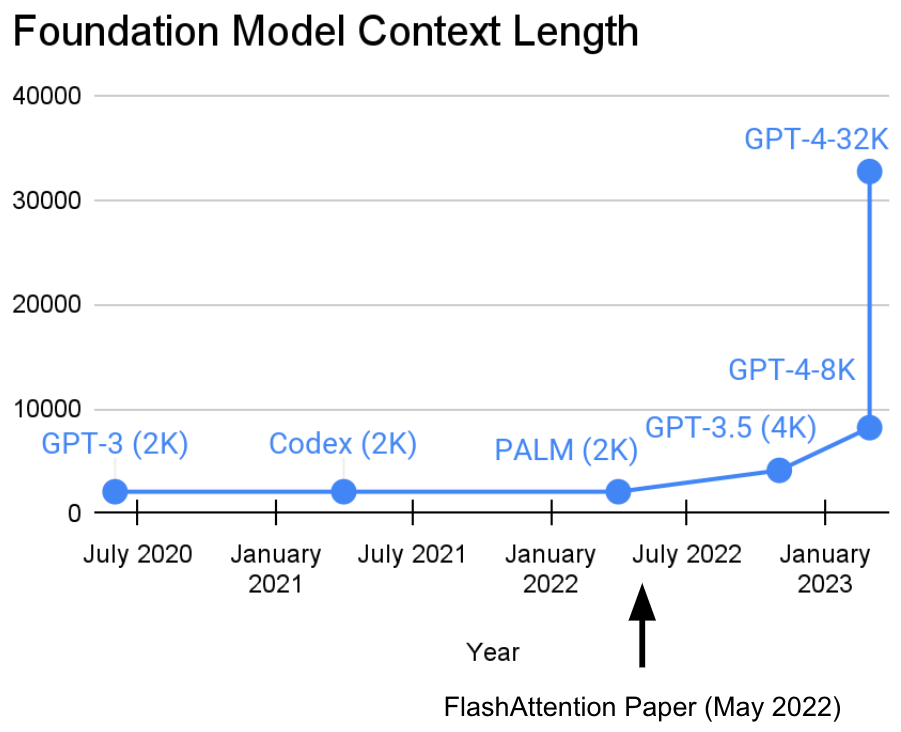
\includegraphics[width=0.75\linewidth]{context.png}
    \end{figure}
\end{frame}

\begin{frame}{Issues with Transformers}

    \begin{itemize}
        \item Training: quadratic time complexity 
        \begin{itemize}
            \item Expensive for long sequence modeling (e.g., video or DNA modeling)
         \end{itemize}
        \item Inference: linear memory complexity
        \begin{itemize}
            \item Requires storing KV cache for each token
            \item High memory burden.
        \end{itemize}
    \end{itemize}    

\end{frame}

\begin{frame}{Revisiting RNNs}
    \begin{figure}
        \centering
        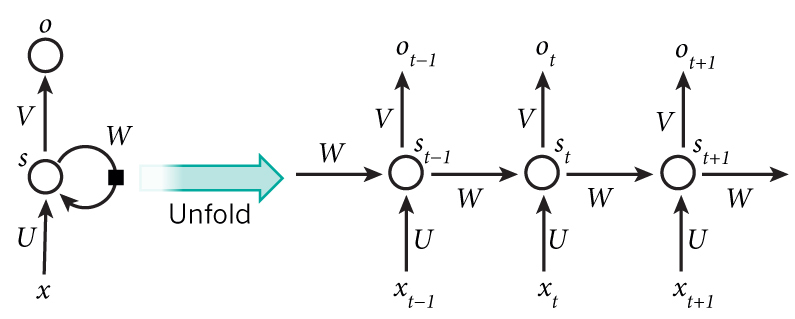
\includegraphics[width=.75\linewidth]{rnn.png}
        % \caption{Transformer architecture}
    \end{figure}
    \begin{itemize}
            \item Training: linear complexity, however, traditional RNNs are not parallelizable.
            \vspace{2mm}
            \item Inference: constant memory
    \end{itemize}
\end{frame}


\begin{frame}{Modern linear recurrent models}
    Use linear recurrence for parallel training
    \vspace{2mm}
    \begin{itemize}
        \item Gated linear RNNs (HGRN, Griffin, ...)
        \item State-space models (S4, Mamba, ...)
        \item Linear attention (RetNet, GLA, xLSTM, DeltaNet, ...)
    \end{itemize}

\end{frame}


\begin{frame}{Modern linear recurrent models}
    Use linear recurrence for parallel training
    \vspace{2mm}
    \begin{itemize}
        \item \textcolor{gray}{Gated linear RNNs (HGRN, Griffin, ...)}
        \item \textcolor{gray}{State-space models (S4, Mamba, ...)}
        \item \color{red}\textbf{Linear attention (RetNet, GLA, xLSTM, DeltaNet, ...)}
    \end{itemize}
    \vspace{2mm}
    \textcolor{black}{Linear attention is the focus of this talk.}
\end{frame}



\begin{frame}{}
    \begin{figure}
        \centering
        \includegraphics[width=.95\linewidth]{hybrid.png}
    \end{figure}
    
    MiniMax-01 (\cite{minimax2025minimax01scalingfoundationmodels}) used hybrid attention: \textcolor{red}{\textbf{7/8}} linear attention layers + \textcolor{red}{\textbf{1/8}} softmax attention layers, with simple linear attention using data-independent decay: Lightning-Attention (\cite{Qin2024VariousLC}).
\end{frame}


\begin{frame}{}
    \centering
    \LARGE
     Linear attention  
\end{frame} 


\begin{frame}{Softmax attention}
     Attention:
    \[
    \begin{aligned}
        \mathrm{Parallel\ training:} &&& \mathbf{O} = \mathrm{softmax}(\mathbf{Q}\mathbf{K}^\top \odot \mathbf{M})\mathbf{V} &&\in \mathbb{R}^{L\times d}   \\
        \mathrm{Iterative\ inference:} &&&\mathbf{o_t} = \sum_{j=1}^t \frac{\exp(\mathbf{q}_t^\top \mathbf{k}_j)}{\sum_{l=1}^t\exp(\mathbf{q}^\top_t \mathbf{k}_l)}\mathbf{v}_j &&\in \mathbb{R}^d 
    \end{aligned}
    \]
    where $\mathbf{M} \in \mathbb{R}^{L \times L}$ is the casual mask:
    \[
    \mathbf{M}_{i,j} = \begin{cases}
        -\infty & \text{if } j > i \\
        1 & \text{if } j \leq i
    \end{cases}
    \]
\end{frame}

\begin{frame}{Linear attention = standard attention - softmax}
    Linear attention (\cite{katharopoulos2020transformers}):
    \[
    \begin{aligned}
        \mathrm{Parallel\ training:} &&& \mathbf{O} = \hcancel[red]{\mathrm{softmax}}(\mathbf{Q}\mathbf{K}^\top \odot \mathbf{M})\mathbf{V} &&\in \mathbb{R}^{L\times d}   \\
        \mathrm{Iterative\ inference:} &&&\mathbf{o_t} = \sum_{j=1}^t \frac{\hcancel[red]{\exp}(\mathbf{q}_t^\top \mathbf{k}_j)}{\hcancel[red]{\sum_{l=1}^t\exp(\mathbf{q}^\top_t \mathbf{k}_l)}}\mathbf{v}_j &&\in \mathbb{R}^d 
    \end{aligned}
    \]
    where $\mathbf{M}$ is the causal mask for linear attention:
    \[
    \mathbf{M}_{i,j} = \begin{cases}
        0 & \text{if } j > i \\
        1 & \text{if } j \leq i
    \end{cases}
    \] 
\end{frame}

\begin{frame}{Equivalent View: Matrix-Valued Hidden States}
    $$ \begin{aligned}  
        \mathbf{o_t} &=  \sum_{j=1}^t (\mathbf{q}_t^\top \mathbf{k}_j) \mathbf{v}_j \\
         &= \sum_{j=1}^t \mathbf{v}_j(\mathbf{k}_j^\top \mathbf{q}_t) &  \mathbf{k}_j^\top \mathbf{q}_t = \mathbf{q}_t^\top \mathbf{k}_j \in \mathbb{R}\\  
        &= {\color{red}\underbrace{(\sum_{j=1}^t \mathbf{v}_j\mathbf{k}_j^\top)}_{\mathbf{S}_t \in \mathbb{R}^{d \times d}}}\mathbf{q}_t & \text{By associativity}
    \end{aligned} $$    
\end{frame}

\begin{frame}{Linear attention = Linear RNN + matrix-valued hidden states}
    Let $\mathbf{S}_t = \sum_{j=1}^t\mathbf{v}_j\mathbf{k}_j^\top \in \mathbb{R}^{d \times d}$ be the matrix-valued hidden state, then:
    $$ \begin{aligned}
        \mathbf{S}_t &= \mathbf{S}_{t-1} + \mathbf{v}_t\mathbf{k}_t^\top &&\in \mathbb{R}^{d \times d}  \\
        \mathbf{o}_t &= \mathbf{S}_t\mathbf{q}_t &&\in \mathbb{R}^d  
    \end{aligned} $$
    
\begin{itemize}
    \item Linear attention implements {\color{red}\textbf{elementwise linear recurrence}}.
    \item Linear attention has a {\color{red}\textbf{matrix-valued hidden state}}, significantly increasing the state size.
\end{itemize}
\end{frame}
\begin{frame}{Challenges in training: the parallel form}
    \centering
    \begin{align*}
        \mathbf{O}= (\mathbf{Q}\mathbf{K}^\top \odot \mathbf{M})\mathbf{V} \in \mathbb{R}^{L\times d} &&
    \end{align*}
    \vspace{2mm}

    The time complexity is still quadratic in sequence length, which is problematic for long sequences.
\end{frame}

\begin{frame}{Challenges in training: the recurrent form}
    \[
    \begin{aligned}
        \mathbf{S}_t &= \mathbf{S}_{t-1} + {\color{blue}\mathbf{v}_t\mathbf{k}_t^\top} &&\in \mathbb{R}^{d \times d}  \\
        \mathbf{o}_t &= {\color{orange}\mathbf{S}_t\mathbf{q}_t} &&\in \mathbb{R}^d  
    \end{aligned}
    \]

     Poor GPU utilization due to:
        \begin{itemize}
            \item Sequential computation limits parallelization opportunities across the sequence dimension.
            \item {\color{blue}Rank-1 outer product updates} and {\color{orange}matrix-vector multiplications} are not optimized for GPU tensor cores, which are designed for dense matrix-multiply operations (typically at least 16x16 matrix sizes).
        \end{itemize}   
    
\end{frame}


\begin{frame}{Chunkwise parallel form}
    \textbf{Chunkwise Form:}
    \begin{itemize}
        \item Interpolates between recurrent and parallel forms.
        \item Splits a sequence of length $L$ into $L/C$ chunks of size $C$:
            \begin{itemize}
                \item When $C=1$, it reduces to the recurrent form.
                \item When $C=L$, it reduces to the parallel form.
            \end{itemize}
        \item  \textbf{Key Property:} Chunkwise form is {\color{red} \textbf{NOT an approximation}}—it computes the exact same output as the original formulation.
        \end{itemize}
\end{frame}

\begin{frame}{Chunkwise parallel form}
    Chunkwise form computes only the {\color{red} \textbf{last hidden state}} per chunk. 
    \\
    Output is derived from:
                \begin{itemize}
                \item {\color{red} \textbf{Recurrent Form:}} Historical context across chunks.
                \item {\color{red} \textbf{Parallel Form:}} Local context within a chunk.
            \end{itemize}
\end{frame}

\begin{frame}{Notations}
 
    \begin{align*}
        \mathbf{S}_{[i]} &:= \mathbf{S}_{iC} \in \mathbb{R}^{d \times d} &&\text{the last hidden state of chunk $i$}, \\
        \mathbf{Q}_{[i]} &= \mathbf{Q}_{iC+1:(i+1)C} \in \mathbb{R}^{C \times d} &&\text{the query block of chunk $i$}. \\
    \end{align*}
    We define $\mathbf{K}_{[i]}, \mathbf{V}_{[i]}, \mathbf{O}_{[i]}$ in a similar way.
\end{frame}

% \begin{frame}
%     \centering
%     \LARGE
%       Linear attention with decay
% \end{frame}


% \begin{frame}{Hardware-efficient training with chunkwise parallel form}
%             \begin{itemize}
%                 \item \textcolor{gray!50}{Sequence of length $L$ divided into $L/C$ chunks of size $C$}
%                 \item \textcolor{gray!50}{Compute only the {last hidden state} of each chunk.}
%                 \item \textcolor{gray!50}{Compute the output from two parts:}
%                 \begin{itemize}
%                     \item \textcolor{gray!50}{Historical context: using recurrent form}
%                     \item \textcolor{gray!50}{Local context: using parallel form}
%                 \end{itemize}
%                 \item When $C=1$, it reduces to recurrent form; when $C=L$, it reduces to parallel form.
%                 \item Chunkwise form is {\color{red} \textbf{NOT an approximation}}, it computes the exact same output.
%             \end{itemize}
    
%             \vspace{2mm}
%             Notation:
%             \begin{align*}
%                 \mathbf{S}_{[i]} &:= \mathbf{S}_{iC} \in \mathbb{R}^{d \times d} &&\text{(Chunk-level hidden state)} \\
%                 \square_{[i]} &= \square_{iC+1:(i+1)C} \in \mathbb{R}^{C \times d} &&\text{(Matrix block for chunk $i$)} \\
%                 &\text{for } \square \in \{\mathbf{Q}, \mathbf{K}, \mathbf{V}, \mathbf{O}\} \\
%             \end{align*}
% \end{frame}



\begin{frame}{}
    % \begin{figure}
    %     \centering
    %     \includegraphics[width=.9\linewidth]{chunk-state.png}
    % \end{figure}
    \definecolor{yellowgreen}{RGB}{154,205,50}    
\definecolor{limeyellow}{RGB}{185,215,40}     
\definecolor{yellowgreenyellow}{RGB}{173,255,47}    

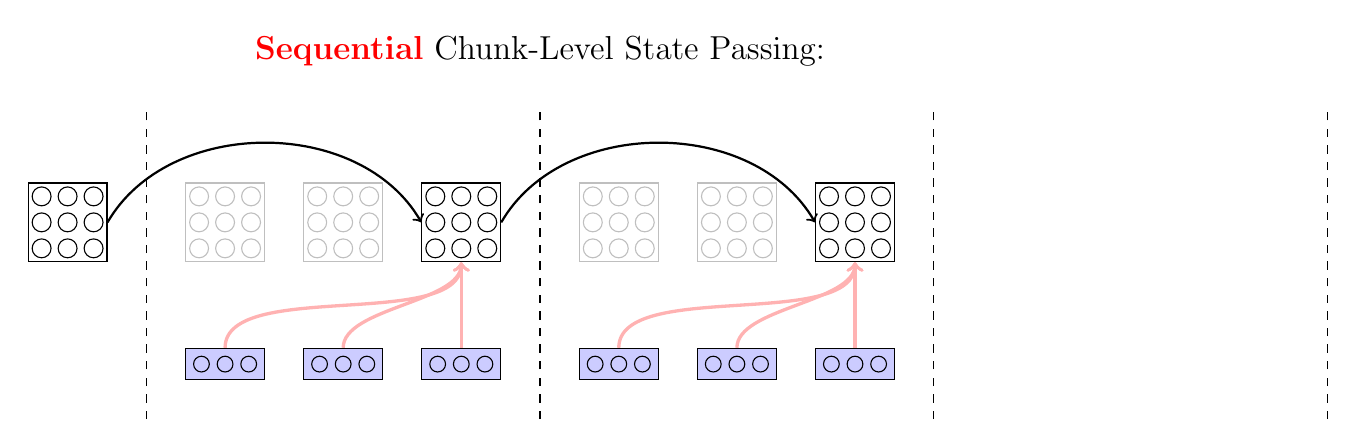
\begin{tikzpicture}
    \foreach \x in {0,5,10,15} {
        \draw[dashed] (\x,-2) -- (\x,2);
    }

        \begin{scope}[shift={(-1.5,0)}]
            \node[draw=black, minimum size=1cm] (grid-0-3) at (0.5,0.5) {};
            \foreach \x in {0,0.33,0.66} {
                \foreach \y in {0,0.33,0.66} {
                    \draw[black] (\x+0.17,\y+0.17) circle (0.12);
                }
            }
        \end{scope}

    \foreach \section [count=\i] in {0.5,5.5} {
        \foreach \offset [count=\j] in {0,1.5} {
            \begin{scope}[shift={(\section+\offset,0)}]
                \node[draw=gray!50, minimum size=1cm] (grid-\i-\j) at (0.5,0.5) {};
                \foreach \x in {0,0.33,0.66} {
                    \foreach \y in {0,0.33,0.66} {
                        \draw[gray!50] (\x+0.17,\y+0.17) circle (0.12);
                    }
                }
            \end{scope}
        }
        
        \begin{scope}[shift={(\section+3,0)}]
            \node[draw=black, minimum size=1cm] (grid-\i-3) at (0.5,0.5) {};
            \foreach \x in {0,0.33,0.66} {
                \foreach \y in {0,0.33,0.66} {
                    \draw[black] (\x+0.17,\y+0.17) circle (0.12);
                }
            }
        \end{scope}
    }
    
    \foreach \section [count=\i] in {0.5,5.5} {
        \begin{scope}[shift={(\section,-1.5)}]
            \foreach \offset [count=\j] in {0,1.5,3} {
                \node[fill=blue!20,draw=black, minimum width=1cm, minimum height=0.4cm] (rect-\i-\j) at (\offset+0.5,0.2) {};
                \foreach \x in {0.2, 0.5, 0.8} {
                    \draw[black] (\offset+\x,0.2) circle (0.1);
                }
                \draw[->,red!30,very thick] (rect-\i-\j.north) to[out=90,in=-90, looseness=0.7] 
                    ([xshift=\j*0cm]grid-\i-3.south);
            }
        \end{scope}
    }
    
% \draw[->,yellowgreen,very thick] (grid-1-3.east) to[bend left=60] node[above,font=\small,xshift=-0.5cm]{$\color{black}\boldsymbol{S}_{[2]}=\boldsymbol{S}_{[1]}{\color{yellowgreen}(\boldsymbol{I}-\boldsymbol{W}_{[2]}^\top \boldsymbol{K}_{[2]})} + {\color{red}\boldsymbol{U}_{[2]}^\top \boldsymbol{K}_{[2]}}$}  (grid-2-3.west);
\draw[->,black, thick] (grid-0-3.east)  to[bend left=60] (grid-1-3.west);
\draw[->,black, thick] (grid-1-3.east)  to[bend left=60] 
node[above,xshift=-1.5cm, yshift=0.5cm,align=center]{
  \textcolor{black}{{\large{\textbf{\color{red}Sequential}} Chunk-Level State Passing:}} \\
%   $\color{black}\boldsymbol{S}_{[i+1]}=\boldsymbol{S}_{[i]}
% + 
%     {\color{blue!50}\colorbox{red!30}{$\boldsymbol{V}_{[i]}^\top \boldsymbol{K}_{[i]}$}}$
} (grid-2-3.west);


\end{tikzpicture}

    \begin{align*}
        &\mathbf{S}_{[t+1]} = \underbrace{\mathbf{S}_{[t]}}_{\mathbb{R}^{d\times d}} + \colorbox{red!30}{$\underbrace{\color{blue!50}\mathbf{V}_{[t]}^\top}_{\mathbb{R}^{d\times C}} \underbrace{\color{blue!50}\mathbf{K}_{[t]}}_{\mathbb{R}^{C\times d}}$} &&\in \mathbb{R}^{d\times d}  \\
    \end{align*}
    Computational Complexity: $\mathcal{O}(Cd^2)$ per chunk and $\mathcal{O}(Ld^2)$ for the entire sequence.
\end{frame}

\begin{frame}{}
    
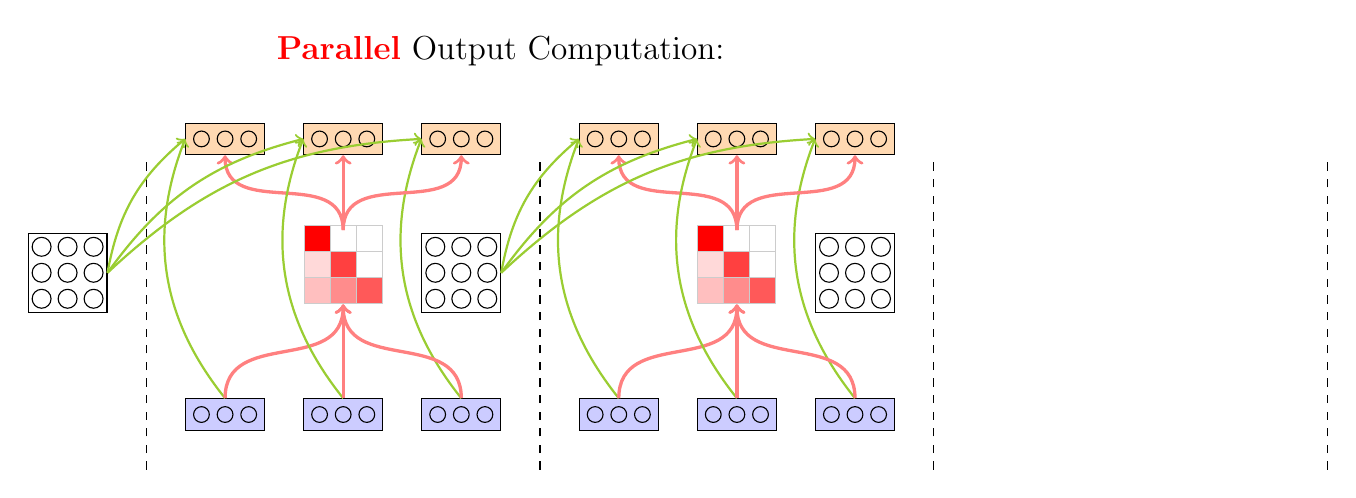
\begin{tikzpicture}[
    box/.style={
        rectangle,
        minimum size=0.5cm,
        draw=black!20
    }
]
    \foreach \x in {0,5,10,15} {
        \draw[dashed] (\x,-2) -- (\x,2);
    }
            \begin{scope}[shift={(-1.5,0)}]
            \node[draw=black, minimum size=1cm] (grid-0-3) at (0.5,0.5) {};
            \foreach \x in {0,0.33,0.66} {
                \foreach \y in {0,0.33,0.66} {
                    \draw[black] (\x+0.17,\y+0.17) circle (0.12);
                }
            }
        \end{scope}


    \foreach \section [count=\i] in {0.5,5.5} {

        % \foreach \offset [count=\j] in {0,1.5} {

     \begin{scope}[shift={(\section+1.5,0.1)}]

        \node[box, fill=red!100, minimum size=0.33cm] at (0.17,0.83) {};
        \node[box, minimum size=0.33cm] at (0.5,0.83) {};
        \node[box, minimum size=0.33cm] at (0.83,0.83) {};
        
        \node[box, fill=red!15, minimum size=0.33cm] at (0.17,0.5) {};
        \node[box, fill=red!75, minimum size=0.33cm] at (0.5,0.5) {};
        \node[box, minimum size=0.33cm] at (0.83,0.5) {};
        

        \node[box, fill=red!25, minimum size=0.33cm] at (0.17,0.17) {};
        \node[box, fill=red!45, minimum size=0.33cm] (attn-\i)at (0.5,0.17) {};
        \node[box, fill=red!65, minimum size=0.33cm] at (0.83,0.17) {};
    \end{scope}

        \begin{scope}[shift={(\section+3,0)}]
            \node[draw=black, minimum size=1cm] (grid-\i-3) at (0.5,0.5) {};
            \foreach \x in {0,0.33,0.66} {
                \foreach \y in {0,0.33,0.66} {
                    \draw[black] (\x+0.17,\y+0.17) circle (0.12);
                }
            }
        \end{scope}
    }
    

    \foreach \section [count=\i] in {0.5,5.5} {
        \begin{scope}[shift={(\section,-1.5)}]

            \foreach \offset [count=\j] in {0,1.5,3} {
                \node[draw=black, fill=blue!20, minimum width=1cm, minimum height=0.4cm] (rect-\i-\j) at (\offset+0.5,0.2) {};

                \foreach \x in {0.2, 0.5, 0.8} {
                    \draw[black] (\offset+\x,0.2) circle (0.1);
                }
                \node[draw=black, minimum width=1cm, minimum height=0.4cm,fill=orange!30] (upper-rect-\i-\j) at (\offset+0.5,0.2+3.5) {};
                \foreach \x in {0.2, 0.5, 0.8} {
                    \draw[black] (\offset+\x,0.2+3.5) circle (0.1);
                }
                
            
    \pgfmathsetmacro{\prevsection}{\i-1}
\draw[->, yellowgreen, thick] 
    (grid-\the\numexpr\i-1\relax-3.east) 
    to[bend left=20] 
    (upper-rect-\i-\j.west);

\draw[->, yellowgreen, thick] 
    (rect-\i-\j.north) 
    to[bend left=30] 
    (upper-rect-\i-\j.west);

\draw[->,red!50,very thick] (rect-\i-\j.north) to[out=90,in=-90,looseness=1.2] (attn-\i.south);

\draw[->,red!50,very thick] ([yshift=0.6cm]attn-\i.north) to[out=90,in=-90,looseness=1.2] (upper-rect-\i-\j.south);

}

\ifnum\i>1
\fi

        \end{scope}
    }
    
\node[above=0.25cm,xshift=-3cm,align=center] at (upper-rect-2-2.north) {
  \textcolor{black}{\large{\textbf{\color{red}Parallel} Output Computation:}} \\
%   ${\color{orange}\mathbf{O}_{[i]}}=\colorbox{yellowgreen!30}{${\color{blue!50}\mathbf{Q}_{[i]}}\mathbf{S}_{[i]}^\top$}+\colorbox{red!30}{\color{blue!50}$\left({\mathbf{Q}_{[i]}\mathbf{K}_{[i]}^\top \odot \mathbf{M}}\right)\mathbf{V}_{[i]}$}$
};

\end{tikzpicture}

    \vspace{-3mm}
    \begin{align*}
        {\color{orange}\mathbf{O}_{[t]}} = \colorbox{yellowgreen!30}{$\underbrace{{\color{blue!50}\mathbf{Q}_{[t]}}\mathbf{S}_{[t]}^\top}_{\text{inter-chunk}:\mathbf{O}_{[t]}^{\text{inter}}}$} + \colorbox{red!30}{$\underbrace{({\color{blue!50}\mathbf{Q}_{[t]}\mathbf{K}_{[t]}^\top \odot \mathbf{M}}){\color{blue!50}\mathbf{V}_{[t]}}}_{\text{intra-chunk}:\mathbf{O}_{[t]}^{\text{intra}}}$} \in \mathbb{R}^{C\times d}
    \end{align*}

    Computational Complexity: $\mathcal{O}(C^2d+Cd^2)$ per chunk. $\mathcal{O}(Ld^2+LCd)$ for the entire sequence.
\end{frame}
\begin{frame}{Chunkwise parallel form}
    \begin{itemize}
        \item \textbf{\textcolor{black}{Total complexity}}: $\mathcal{O}(Ld^2 + LdC)$, achieving \textbf{\textcolor{red}{subquadratic complexity}} in sequence length when $C$ is small.
        \item \textbf{\textcolor{black}{Practical settings}}: $C$ is typically set to $\{64, 128, 256\}$.
        \item \textbf{\textcolor{black}{Extensibility}}: Can be generalized to \textbf{\textcolor{red}{linear attention with decay and delta rule}} (to be discussed later).
        \item \textbf{\textcolor{black}{Adoption}}: The de facto standard for training modern linear attention models, including:
        \begin{itemize}
            \item \textbf{\textcolor{red}{Mamba2}}, \textbf{\textcolor{red}{Based}}, \textbf{\textcolor{red}{GLA}}, \textbf{\textcolor{red}{DeltaNet}}, \textbf{\textcolor{red}{Lightning Attention}}, \textbf{\textcolor{red}{mLSTM}}, and others.
        \end{itemize}
    \end{itemize}
\end{frame}


% \begin{frame}
%     \frametitle{Flash linear attention: I/O-aware chunkwise parallel form}
%     \begin{figure}
%         \centering
%         \includegraphics[width=.8\linewidth]{fla.png}
%     \end{figure}
%     \begin{itemize}
%         \item In step1: only recurrent state is computed, reducing the total FLOPs spent in recurrence.
%         \item In step2: outputs are computed in parallel with kernel fusion to reduce I/O.
%     \end{itemize}
% \end{frame}

\begin{frame}{Flash linear attention}
 \begin{figure}
    \centering
    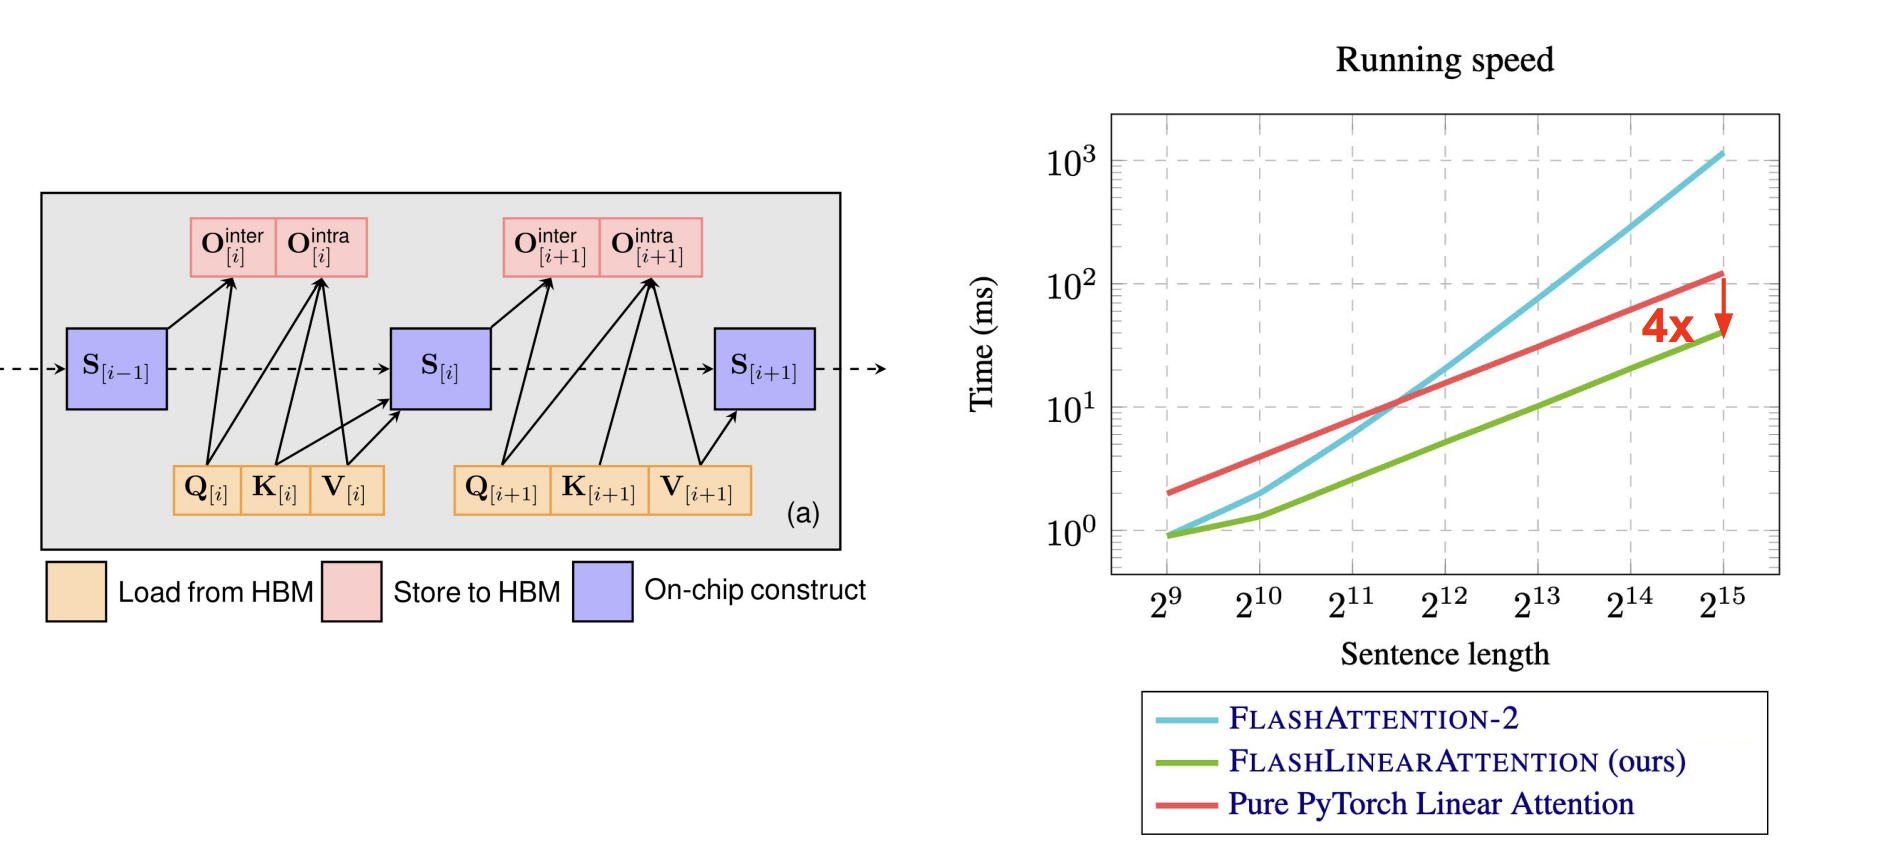
\includegraphics[width=1.1\linewidth]{fla-speed.png}
 \end{figure}
 \vspace{2mm} 
   I/O optimization significantly improves the wall-clock time.
\end{frame}

\begin{frame}{Flash linear attention}
    \begin{figure}
        \centering
        
\includegraphics[width=.9\linewidth]{fla-repo.png}
    \end{figure}
    The Flash Linear Attention library provides hardware-efficient implementation of various linear attention models.
    \begin{itemize}
        \item RetNet, GLA, Based, HGRN2, RWKV6, GSA, Mamba2, DeltaNet, Gated DeltaNet, RWKV7  ...
    \end{itemize}
\end{frame}

\begin{frame}{Summary}
    \begin{itemize}
        \item Linear attention = Softmax attention - softmax.
        \item Linear attention = Linear RNN + {\color{red}{matrix-valued hidden state}}.
        \item The chunkwise parallel form is more {\color{red}{hardware-friendly}} than the recurrent and parallel forms.
        \item Flash Linear Attention is an {\color{red}{I/O-aware}} implementation of the chunkwise parallel form.
    \end{itemize}
\end{frame}

\begin{frame}{}
    \centering
    \LARGE
     Linear attention with decay
\end{frame} 



\begin{frame}{Linear attention is not enough}
    \begin{align*}
        \mathbf{S}_t &= \mathbf{S}_{t-1} + \mathbf{v}_t\mathbf{k}_t^\top &&\in \mathbb{R}^{d \times d}  \\
        \mathbf{o}_t &= \mathbf{S}_t\mathbf{q}_t &&\in \mathbb{R}^d  
    \end{align*}
    Vanilla linear attention models significantly underperform Transformers in language modeling.
    \begin{itemize}
        \item Recent tokens are more important than distant tokens in language modeling.
        \item Vanilla linear attention does not have any mechanism to weigh recent tokens more.
    \end{itemize}
    % \begin{itemize}
    %     \item Training instability: no decay.
    %     \item Lack positional encoding: the hidden state is like a bag of key-value word memory.
    % \end{itemize}
    % \begin{itemize}
    %     \item No positional encoding: the hidden state is like a bag of key-value word memory.
    %     \item No decay: the hidden state value could explode due to cumulative sum without decay.
    % \end{itemize}
        % \begin{itemize}
        %     \item {\color{red}{\textbf{Instability:}}} the hidden state value could explode due to cumulative sum without decay

        % \end{itemize}
\end{frame}


\begin{frame}{Linear attention with data-independent decay}
    \begin{align*}
        \mathbf{S}_t &= {\color{red}\gamma} \mathbf{S}_{t-1} + \mathbf{v}_t\mathbf{k}_t^\top &&\in \mathbb{R}^{d \times d}  \\
        \mathbf{o}_t &= \mathbf{S}_t\mathbf{q}_t &&\in \mathbb{R}^d  
    \end{align*}
    \begin{itemize}
        \item ${\color{red}\gamma}$ is a constant exponential decay factor ${\color{red}0 < \gamma < 1}$.
        \item Works well in practice: RetNet (\cite{sun2023retentive}), Lightning Attention (\cite{Qin2024VariousLC})
        % \item Lacking selectivity: a potential issue.
    \end{itemize}
\end{frame}



\begin{frame}{Linear attention with data-dependent decay}
    \begin{align*}
        \mathbf{S}_t &= {\color{red}\gamma_t} \mathbf{S}_{t-1} + \mathbf{v}_t\mathbf{k}_t^\top &&\in \mathbb{R}^{d \times d}  \\
        \mathbf{o}_t &= \mathbf{S}_t\mathbf{q}_t &&\in \mathbb{R}^d  
    \end{align*}
    \begin{itemize}
        \item ${\color{red}{\gamma_t} \in (0, 1)}$ is a data-dependent decay term that is a function of $\mathbf{x}_t$.
        \item Enables dynamic control of memory retention/forgetting based on input data.
        \item Examples: Mamba2 (\cite{mamba2}), mLSTM (\cite{beck2024xlstm}), Gated Retention (\cite{sun2024you}).
    \end{itemize}
\end{frame}

\begin{frame}{The parallel form for linear attention with decay}
    \begin{align*}
        \mathbf{S}_t &= {\color{red}\gamma_t} \mathbf{S}_{t-1} + \mathbf{v}_t\mathbf{k}_t^\top &&\in \mathbb{R}^{d \times d}  \\
        \mathbf{o}_t &= \mathbf{S}_t\mathbf{q}_t &&\in \mathbb{R}^d  
    \end{align*}

    Linear attention with decay has the following parallel form:
    \begin{align*}
        \mathbf{O} &= (\mathbf{Q}\mathbf{K}^\top \odot {\color{red} \mathbf{D}})\mathbf{V} \in \mathbb{R}^{L\times d} && \\
        \color{red} \mathbf{D}_{i,j} &= \begin{cases}
            \prod_{m=j+1}^i {\color{red}\gamma_m} & \text{if } i > j \\
            1 & \text{if } i = j \\
            0 & \text{otherwise}
        \end{cases}
    \end{align*}

     The duality between recurrent and parallel forms is referred to as {\color{blue}state space duality (SSD)} in Mamba2 (\cite{mamba2}).
\end{frame}

% \begin{frame}{The chunkwise parallel form for linear attention with decay}
%     \begin{align*}
%         \mathbf{S}_t &= {\color{red}\gamma_t} \mathbf{S}_{t-1} + \mathbf{v}_t\mathbf{k}_t^\top &&\in \mathbb{R}^{d \times d} &&& \mathbf{o}_t &= \mathbf{S}_t\mathbf{q}_t &&\in \mathbb{R}^d 
%     \end{align*}
%     Linear attention with decay has the following chunkwise form:
%     \begin{align*}
%         \mathbf{S}_{[t]} &= {\color{red}\beta_{tC}} \mathbf{S}_{[t-1]}  +  (\mathbf{V}_{[t]} \odot {\color{red}\frac{\beta_{tC}}{\beta_{[t]}}[:,\, \text{None}]})^\top \mathbf{K}_{[t]} &&\in \mathbb{R}^{d \times d}  \\
%         \mathbf{O}_{[t]} &= \underbrace{(\mathbf{Q}_{[t]} \mathbf{S}_{[t]}^\top) \odot {\color{red}\beta_{[t]}[:,\, \text{None}]}}_{\text{inter-chunk}} + \underbrace{(\mathbf{Q}_{[t]} \mathbf{K}_{[t]}^\top \odot {\color{red}\mathbf{D}_{[t]}}) \mathbf{V}_{[t]}}_{\text{intra-chunk}} &&\in \mathbb{R}^{C \times d} 
%     \end{align*}
%     The chunkwise form with decay is {\color{blue}\textbf{mathematically equivalent}} to Mamba2's {\color{red}\textbf{SSD block decomposition algorithm}}.
% \end{frame}

% \begin{frame}{The chunkwise parallel form for linear attention with decay}
%     \begin{align*}
%         \mathbf{S}_{[t]} &= {\color{red}\beta_{tC}} \mathbf{S}_{[t-1]}  +  (\mathbf{V}_{[t]} \odot {\color{red}\frac{\beta_{tC}}{\beta_{[t]}}[:,\, \text{None}]})^\top \mathbf{K}_{[t]} &&\in \mathbb{R}^{d \times d}  \\
%         \mathbf{O}_{[t]} &= \underbrace{(\mathbf{Q}_{[t]} \mathbf{S}_{[t]}^\top) \odot {\color{red}\beta_{[t]}[:,\, \text{None}]}}_{\text{inter-chunk}} + \underbrace{(\mathbf{Q}_{[t]} \mathbf{K}_{[t]}^\top \odot {\color{red}\mathbf{D}_{[t]}}) \mathbf{V}_{[t]}}_{\text{intra-chunk}} &&\in \mathbb{R}^{C \times d} 
%     \end{align*}
%     \begin{itemize}
%         \item<1-1> $\mathbf{S}_{[t]}:=\mathbf{S}_{tC} \in \mathbb{R}^{d \times d}$. $\square_{[t]}:=\square_{tC+1:(t+1)C} \in \mathbb{R}^{C \times d}$ for $\square \in \{\mathbf{Q}, \mathbf{K}, \mathbf{V}, \mathbf{O}\}$.
%         \item<1-1> ${\color{red} \beta_{[t]} \in \mathbb{R}^{C}}$ represents the cumulative decay values within chunk $t$, where the $i$-th element is ${\color{red}(\beta_{[t]})_i= \beta_{tC+i}= \prod_{m=tC+1}^{tC+i}\gamma_m \in \mathbb{R}}$
%         \item<1-1> ${\color{red}(\mathbf{D}_{[t]})_{i,j}} = \begin{cases}
%             {\color{red}\prod_{m=tC+i+1}^{tC+j} \gamma_m} & \text{if } i < j \\
%             1 & \text{if } i = j \\
%             0 & \text{otherwise}  
%         \end{cases} \qquad \in \mathbb{R}^{C \times C}$ 
%     \end{itemize}

%     We highlight the decay-related terms in red and if we remove these red terms, we recover the chunkwise form of vanilla linear attention.

% \end{frame}



% \begin{frame}{The chunkwise parallel form for linear attention with decay}
%     \begin{align*}
%         \mathbf{S}_t &= {\color{red}\gamma_t} \mathbf{S}_{t-1} + \mathbf{v}_t\mathbf{k}_t^\top &&\in \mathbb{R}^{d \times d} &&& \mathbf{o}_t &= \mathbf{S}_t\mathbf{q}_t &&\in \mathbb{R}^d 
%     \end{align*}
%     Linear attention with decay has the following chunkwise form:
%     \begin{align*}
%         \mathbf{S}_{[t]} &= {\color{red}\beta_{Ct}} \mathbf{S}_{[t-1]}  +  (\mathbf{V}_{[t]} \odot {\color{red}\frac{\beta_{tC}}{\beta_{[t]}}[:,\, \text{None}]})^\top \mathbf{K}_{[t]} &&\in \mathbb{R}^{d \times d}  \\
%         \mathbf{O}_{[t]} &= \underbrace{(\mathbf{Q}_{[t]} \mathbf{S}_{[t]}^\top) \odot {\color{red}\beta_{[t]}[:,\, \text{None}]}}_{\text{inter-chunk}} + \underbrace{(\mathbf{Q}_{[t]} \mathbf{K}_{[t]}^\top \odot {\color{red}\mathbf{D}_{[t]}}) \mathbf{V}_{[t]}}_{\text{intra-chunk}} &&\in \mathbb{R}^{C \times d} 
%     \end{align*}
%     \begin{itemize}
%         \item Preserves matrix-multiply structure with minimal overhead when incorporating decay
%         \item As fast as vanilla linear attention's chunkwise form
%         \item Equivalent to Mamba2's block decomposition-based {\color{red} \textbf{SSD algorithm}} (\cite{mamba2}).
%     \end{itemize}

% \end{frame}






\begin{frame}{Linear attention with more fine-grained decay}

    \begin{align*}
        \mathbf{S}_t &= {\color{red}\mathbf{G}_t} \odot \mathbf{S}_{t-1} + \mathbf{v}_t\mathbf{k}_t^\top &&\in \mathbb{R}^{d \times d}  \\
        \mathbf{o}_t &= \mathbf{S}_t\mathbf{q}_t &&\in \mathbb{R}^d  
    \end{align*}
    % where {\color{red}$\mathbf{G}_t \in \mathbb{R}^{d \times d}$} is a data-dependent gate matrix. 

    \textbf{Condition} for having the parallel form (\cite{gla}):
    \[{\color{red}\mathbf{G}_t = \boldsymbol{\beta}_t\boldsymbol{\alpha}_t^\top \in \mathbb{R}^{d\times d}, \quad \boldsymbol{\alpha}_t, \boldsymbol{\beta}_t \in \mathbb{R}^d}
    \]


    \begin{itemize}
        \item Mamba-1 does not conform to this structure, making it impractical to leverage tensor cores.
        \item It is often to set $\boldsymbol{\beta}_t = \mathbf{1}$ for efficiency considerations, examples: GLA (\cite{gla}), RWKV6 (\cite{rwkv6}).
    \end{itemize}

%      $\mathbf{G}_t = \boldsymbol{\beta}_t\boldsymbol{\alpha}_t^\top}, \quad \boldsymbol{\alpha}_t, \boldsymbol{\beta}_t \in \mathbb{R}^d$, 
%     Examples:
%         \item \textbf{GLA} (\cite{gla}): 
%             \[
%             {\color{red}\mathbf{G}_t = \boldsymbol{\beta}_t\boldsymbol{\alpha}_t^\top}, \quad \boldsymbol{\alpha}_t, \boldsymbol{\beta}_t \in \mathbb{R}^d
%             \]
%             \vspace{-5mm}
%             \begin{itemize}
%                 \item Outer product structure enables efficient training with chunkwise parallel form.
%             \end{itemize}
%             \item \textbf{Mamba-1} (\cite{Gu2023MambaLS}): 
%             \[
%             {\color{red}\mathbf{G}_t = \exp\left(-(\boldsymbol{\Delta}_t \mathbf{1}^\top) \odot \exp(\mathbf{A})\right)}, \mathbf{A} \in \mathbb{R}^{d \times d}, \boldsymbol{\Delta}_t \in \mathbb{R}^{d} 
%             \]
%             \vspace{-5mm}
%             % \begin{itemize}
%                 % \item  is data-independent. $\boldsymbol{\Delta}_t \in \mathbb{R}^{d}$ is data-dependent.
%                 % \item Non-outer product structure makes it challenging to formulate in chunkwise form.
%             % \end{itemize}
%     \end{itemize}
\end{frame}

\begin{frame}{Summary}
    \begin{itemize}
        \item Language modeling has a strong recency bias.
        \item Decay helps bridge the perplexity gap between linear and softmax attention.
        \item Fine-grained decay improves performance but faces scaling challenges.
        \item Outer-product decay structure enables efficient chunkwise training.
    \end{itemize}
\end{frame}

% \begin{frame}{Linear attention with more fine-grained decay}
%     \begin{align*}
%         \mathbf{S}_t &= {\color{red}\mathbf{G}_t} \odot \mathbf{S}_{t-1} + \mathbf{v}_t\mathbf{k}_t^\top &&\in \mathbb{R}^{d \times d}  \\
%         \mathbf{o}_t &= \mathbf{S}_t\mathbf{q}_t &&\in \mathbb{R}^d  
%     \end{align*}
%     \begin{itemize}
%         \item Full form: {\color{red}$\mathbf{G}_t = \boldsymbol{\beta_t}\boldsymbol{\alpha_t}^\top$}
%             \begin{itemize}
%                 \item Examples: Decaying fast weight (\cite{mao-2022-fine})
%                 \item Hardware-efficient training with chunkwise parallel form (\cite{gla}).
%             \end{itemize}
%         \item  A simpler choice: {\color{red}$\mathbf{G}_t = \mathbf{1}\boldsymbol{\alpha_t}^\top$} by setting {\color{red}$\boldsymbol{\beta_t} = \mathbf{1}$}
%         \begin{itemize}
%             \item Faster than the full form case, but still slower than linear attention with scalar-valued decay (e.g., Lightning Attention, Mamba2).
%             \item Examples: GLA (\cite{gla}), RWKV6 (\cite{rwkv6}), MetaLA (\cite{meta_la}), HGRN2 (\cite{hgrn2}), GSA (\cite{zhang2024gated})        
%         \end{itemize}
%     \end{itemize}
% \end{frame}



\begin{frame}{}
    \centering
    \LARGE
    Toward more expressive update rule
\end{frame}

\begin{frame}{Linear attention as a fast weight programming perspective}
\[
    \mathbf{o}_t = \mathbf{S}_t \mathbf{q}_t
\]
We can think of the recurrent hidden state $\mathbf{S}_t$ as a fast weight matrix that maps input $\mathbf{q}_t$ to output $\mathbf{o}_t$ and is updated as it goes:
\[\mathbf{S}_t = \mathbf{S}_{t-1} + \mathbf{v}_t\mathbf{k}_t^\top\]

\end{frame}


% \begin{frame}{Gated Linear Attention: Motivation}
%     \[
%         \begin{aligned}
%             \mathbf{S}_t &= \mathbf{S}_{t-1} + \mathbf{v}_t\mathbf{k}_t^\top &&\in \mathbb{R}^{d \times d}  \\
%             \mathbf{o}_t &= \mathbf{S}_t\mathbf{q}_t &&\in \mathbb{R}^d  
%         \end{aligned}
%         \]    
% \begin{itemize}
%     \item<1-> The cumulative sum tend to explode the hidden state, leading to unstable training and poor language modeling performance.
%     \item<2-> RetNet uses data-independent decay, narrowing down the performance gap, but still underperforming Transformers.
%     \item<3-> Forget gate has been the `missing piece' in linear attention.
% \end{itemize}
% \end{frame}

% \begin{frame}{Gated Linear Attention: Full Form}
%     \begin{align*}
%         \mathbf{S}_t = \mathbf{G}_t \odot \mathbf{S}_{t-1} + \mathbf{v}_t \mathbf{k}_t^\top
%     \end{align*}
%     where $\mathbf{G}_t = \boldsymbol{\beta_t}\boldsymbol{\alpha_t}^\top$ is the gate matrix.
% \begin{itemize}
%     \item Both input $\mathbf{v}_t \mathbf{k}_t^\top$ and gate matrix $\mathbf{G}_t$ are in outer product form
%     \item This structure enables efficient computation via matrix multiplication
% \end{itemize}
% \end{frame}

% \begin{frame}{Gated Linear Attention: Simplified Form}
    
%     When $G_t = \mathbf{1} \boldsymbol{\alpha_t}^\top$:

%     \begin{align*}
%       \mathbf{O}_t =   ((\mathbf{Q} \odot \mathbf{A}) (\mathbf{K} \odot \mathbf{A}^{-1}) \odot \mathbf{M}) \mathbf{V}
%     \end{align*}
%     where $\mathbf{A}_t = \bigodot_{i=1}^t \alpha_i $ is the cumulative product of decay, and $\mathbf{A}^{-1}$ denotes element-wise inverse (not matrix inverse).
% \\
% \vspace{2mm}
% Balanced between training efficiency and expressiveness. Examples:
% \begin{itemize}
%     \item  GLA (\cite{gla})
%     \item  HGRN2 (\cite{hgrn2})
%     \item  RWKV6 (\cite{rwkv6})
%     \item  GSA (\cite{zhang2024gated})
%     \item  MetaLA (\cite{meta_la})
%     \item  ...
% \end{itemize}


% \end{frame}

% \begin{frame}{Gated Linear Attention: Simplest Form}
%     When $G_t = \alpha_t \mathbf{1} \mathbf{1}^\top$:
%     \begin{align*}
%         \mathbf{O}_t &= \left(\mathbf{Q} \mathbf{K}^\top \odot \mathbf{D} \right)\mathbf{V}, \\
%         \mathbf{D}_{ij} &= \begin{cases}
%             \prod_{k=j+1}^{i} \alpha_k & \text{if } i \geq j \\
%             0 & \text{otherwise}
%         \end{cases}
%     \end{align*}
%     Maximum training efficiency, but limited expressiveness. Examples:
%     \begin{itemize}
%         \item Mamba2 (\cite{mamba2})
%         \item xLSTM (\cite{beck2024xlstm})
%         \item Gated RetNet (\cite{Sun2024YouOC})
%     \end{itemize}


% \end{frame}

% \begin{frame}{}
%     \centering
%     \LARGE
%      Modern RNNs Gen3:\\
%     \vspace{1cm} \Large More expressive update rule beyond ELR
% \end{frame}

% \begin{frame}{ELR is of limited expressiveness}

%     \vspace{.5cm}
%     \begin{itemize}
%         \item ELR models fall under the complexity of $TC^0$ (\cite{Merrill2024TheIO}).
%     \end{itemize}
%     \begin{figure}
%     \centering
%     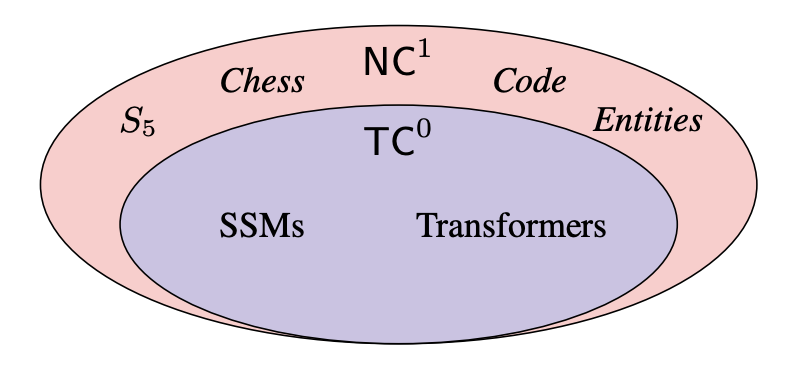
\includegraphics[width=0.5\linewidth]{tc0.png}
%     \caption{The figure is from \cite{Merrill2024TheIO}.}
%     \end{figure}
% \end{frame}

% \begin{frame}{ELR is of limited expressiveness}
%     \vspace{.5cm}
%     \begin{itemize}
%         \item ELR models suffer from in-context associative recall.
%     \end{itemize}
%     \begin{figure}
%             \centering
%             \includegraphics[width=.5\linewidth]{mamba-copy.png}
%         \caption{The figure is from \cite{jelassi2024repeat}. Mamba greatly underperforms Transformers on in-context sentence copying.}
%     \end{figure}
% \end{frame}


% \begin{frame}{ELR is of limited expressiveness}
%     \vspace{.5cm}
%     \begin{itemize}
%         \item ELR models suffer from in-context learning.
%     \end{itemize}
%     \begin{figure}
%             \centering
%             \includegraphics[width=.8\linewidth]{icll.png}
%         \caption{The figure is from \cite{}. Mamba greatly underperforms Transformers on in-context sentence copying.}
%     \end{figure}
% \end{frame}


\begin{frame}{Linear attention as a fast weight programming perspective}
    \resizebox{\linewidth}{!}{
    \begin{tikzpicture}[
        node distance=4.5cm,
        box/.style={
            rectangle,
            draw,
            minimum height=1cm,
            minimum width=1.2cm,
            thick,
            fill=blue!10
        },
        arrow/.style={->,>=latex,thick},
        small box/.style={
            rectangle,
            draw,
            minimum width=0.8cm,
            minimum height=0.8cm,
            inner sep=2pt,
            font=\sffamily,
            fill=orange!10
        },
        values box/.style={
            rectangle,
            draw,
            pattern=north west lines,
            pattern color=green!40,
            fill=green!10,
            minimum size=0.8cm,
            thick
        },
        pink box/.style={
            rectangle,
            draw=pink!80!red,
            thick,
            minimum height=1.2cm,
            minimum width=3cm,
            fill=pink!20,
        },
        weight box/.style={
            rectangle,
            draw=blue!60,
            thick,
            minimum height=1cm,
            minimum width=8cm,
            align=center,
            fill=blue!5
        },
        fast weight box/.style={
            rectangle,
            draw=orange,
            thick,
            fill=orange,
            fill opacity=0.3,
            draw opacity=0.5,
            text opacity=1
        }
    ]
    
    \begin{scope}[on background layer]
        % 状态框
        \node (M1) at (3, 0) {};
        \node[box] (M2) at (4.5,0) {$\mathbf{S}_{t-1}$};
        \node[box] (M3) at (9,0) {$\mathbf{S}_{t}$};
        \node[box] (M4) at (13.5,0) {$\mathbf{S}_{i+1}$};
        
        % Fast weights包裹框
        \path (2.5, 0) -- (M4.south east) node[midway,yshift=-0.5cm] (note) {\small\textbf{\textcolor{orange}{(rapidly changes at each time step)}}};
        \node[fast weight box,fit=(M1)(M2)(M3)(M4)(note),inner sep=10pt] (fastbox) {};
    \end{scope}
    
    % 输入层
    \node[left] at (0.6,6) {\sffamily\Large\bfseries inputs}; 
    \node[box] (X1) at (4.5,6) {$\mathbf{x}_{t-1}$};
    \node[box] (X2) at (9,6) {$\mathbf{x}_t$};
    \node[box] (X3) at (13.5,6) {$\mathbf{x}_{t+1}$};
    
    % Slow weights层
    \node[left] at (0.6,4) {\sffamily\Large\bfseries slow weights};
    \node[weight box] (W) at (9,4) {$\mathbf{W}_q, \mathbf{W}_k, \mathbf{W}_v$\\\small(shared across time steps)};
    
    % 状态间连接
    \draw[arrow] (1.5,0) -- (M2) coordinate[pos=0.95] (M12);
    \draw[arrow] (M2) -- (M3) coordinate[pos=0.95] (M23);
    \draw[arrow] (M3) -- (M4) coordinate[pos=0.95] (M34);
    \draw[arrow] (M4) -- (15.5,0) coordinate[pos=0.95];
    
    % KVQ组
    \foreach \x/\pos/\endpoint/\i/\m in {4.5/a/M12/{t-1}/M2,9/b/M23/t/M3,13.5/c/M34/{t+1}/M4} {
        \node[pink box] (PB\pos) at (\x,2) {};
        \node[small box] (K\pos) at ($(\x,2)+(-0.8,0)$) {$\mathbf{k}_{\i}$};
        \node[small box] (V\pos) at (\x,2) {$\mathbf{v}_{\i}$};
        \node[small box] (Q\pos) at ($(\x,2)+(0.8,0)$) {$\mathbf{q}_{\i}$};
        
        \draw[->,thick] (K\pos.south) to[bend right=45] (\endpoint);
        \draw[->,thick] (V\pos.south) to[bend right=25] (\endpoint);
        \draw[->,thick] (Q\pos.south) to[out=-90,in=90] (\m.north);
    }
    
    % 输入到权重的连接
    \foreach \x in {4.5,9,13.5} {
        \node (X) at (\x,6) {};
        \node (PB) at (\x,2) {};
        \draw[->,thick,blue!60] (X) to[out=-60,in=90] (W);
        \draw[->,thick,blue!60] (W) to[out=-90,in=90] (PB);
    }
    
    % 输出层
    \node[values box] (V2) at (4.5,-2.2) {$\mathbf{o}_{t-1}$};
    \node[values box] (V3) at (9,-2.2) {$\mathbf{o}_{t}$};
    \node[values box] (V4) at (13.5,-2.2) {$\mathbf{o}_{t+1}$};
    
    % 标签
    \node[left] at (0.6,2) {\sffamily\Large\bfseries queries/keys/values};
    \node[left] at (0.6,-2.2) {\sffamily\Large\bfseries outputs};
    \node[left] at (0.6,0) {\sffamily\Large\bfseries fast weights};
    
    % 输出连接
    \draw[arrow] (M2) -- (V2);
    \draw[arrow] (M3) -- (V3);
    \draw[arrow] (M4) -- (V4);
    
    \end{tikzpicture}
    
    }
        
    % - Implements a form of working memory    
%     The hidden state matrix $\mathbf{S}_t$ is a fast weight matrix that is updated at each timestep:
%     \begin{align*}
%         \mathbf{S}_t &= \mathbf{S}_{t-1} + \mathbf{v}_t \mathbf{k}_t^\top
%     \end{align*}
%     \vspace{2mm}
    
%     The fast weight matrix is used to map inputs $\mathbf{q}_t$ into outputs $\mathbf{o}_t$:
% \begin{align*}
%     \mathbf{o}_t = \mathbf{S}_t \mathbf{q}_t
\vspace{-4mm}
\begin{itemize}
    \item {\color{red}\textbf{Fast Weight}}: $\mathbf{S}_t$ maps $\mathbf{q}_t$ to $\mathbf{o}_t$, updated dynamically during inference  for rapid adaptation.
    \item {\color{red}\textbf{Slow Weight}}: $\mathbf{W}_q$, $\mathbf{W}_k$, and $\mathbf{W}_v$ are fixed during inference and only updated during training (e.g., via gradient descent).
\end{itemize}


% \begin{quote}
%     ``Fast weights provide a neurally plausible way of implementing the type of temporary storage that is required by working memory, while slow weights capture more permanent associations learned over many experiences.''
%     \small{ -- Geoffrey Hinton}
% \end{quote}


\end{frame}

\begin{frame}{The choice of update rule}
    \begin{figure}
        \centering
        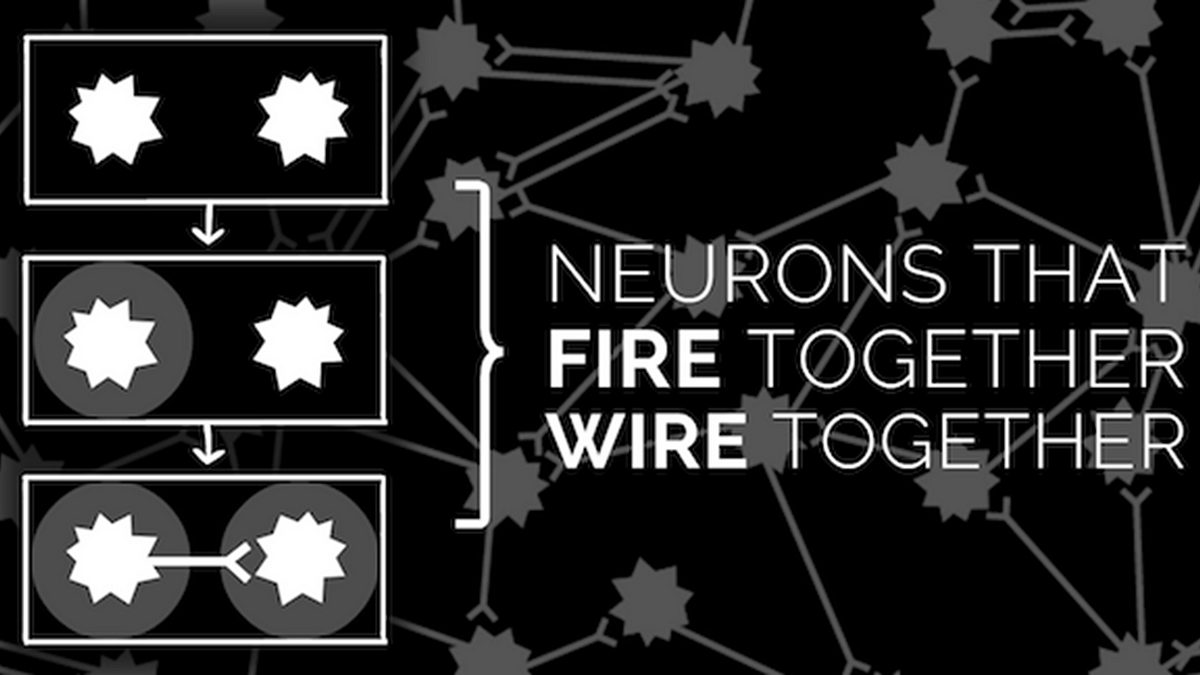
\includegraphics[width=.5\linewidth]{hebbian.png}
        \caption{The principle of Hebbian learning.}
    \end{figure}
    \begin{itemize}
        \item Hebbian update rule: $\mathbf{S}_t = \mathbf{S}_{t-1} + \mathbf{v}_t \mathbf{k}_t^\top$
        \item Delta rule: $\mathbf{S}_t = \mathbf{S}_{t-1} - \beta_t \left(\mathbf{S}_{t-1} \mathbf{k}_t - \mathbf{v}_t\right) \mathbf{k}_t^\top$
        \item ...
    \end{itemize}
    Both Hebbian and delta update rules can be regarded as optimizing online learning objective via {\color{red}test-time SGD}.


\end{frame}
\begin{frame}{Linear Attention: Test-Time Objective}
    \begin{center}
    \begin{tikzpicture}
        \begin{scope}[xshift=3cm]
            \node at (0,3.5) {Maximize alignment};
            \node at (0,3) {= Minimize angle difference + enlarge $|\mathbf{S}\mathbf{k}|$};
            
            \coordinate (O) at (0,0);
            \draw[->,purple,thick] (O) -- (1.75,1.75) coordinate (Mk) node[above] {$\mathbf{S}_{t-1}\mathbf{k}_t$};
            \draw[->,blue,thick] (O) -- (1.5,0.8) coordinate (v) node[right] {$\mathbf{v}_t$};
            
            \draw[->, purple,dashed] (O) -- (3,2.1) node[above] {$\mathbf{S}_{t}\mathbf{k}_t$};
    
            \draw[dashed] (-1,0) -- (2,0);
            \draw[dashed] (0,-1) -- (0,2);
            
            \pic [draw, angle radius=5mm] {angle = v--O--Mk};
        \end{scope}
    \end{tikzpicture}
    \end{center}
\vspace{-10mm}
    \begin{align*}
\hspace*{-1cm}\textbf{Objective: } & \mathcal{L}_t(\mathbf{S}) = -\langle \mathbf{S} \mathbf{k}_t, \mathbf{v}_t \rangle \\[1ex]
\hspace*{-1cm}\textbf{SGD update: } & \mathbf{S}_t = \mathbf{S}_{t-1} - \beta_t \nabla \mathcal{L}_t(\mathbf{S}_{t-1}) = \mathbf{S}_{t-1} + \beta_t \mathbf{v}_t \mathbf{k}_t^\top
    \end{align*}
    \vspace{-6mm}

\end{frame}

\begin{frame}{Linear Attention: Test-Time Objective}
    \begin{center}
        \begin{tikzpicture}
            \begin{scope}[xshift=3cm]
                \node at (0,3.5) {Maximize alignment};
                \node at (0,3) {= Minimize angle difference + enlarge $|\mathbf{S}\mathbf{k}|$};
                
                \coordinate (O) at (0,0);
                \draw[->,purple,thick] (O) -- (1.75,1.75) coordinate (Mk) node[above] {$\mathbf{S}_{t-1}\mathbf{k}_t$};
                \draw[->,blue,thick] (O) -- (1.5,0.8) coordinate (v) node[right] {$\mathbf{v}_t$};
                
                \draw[->, purple,dashed] (O) -- (3,2.1) node[above] {$\mathbf{S}_{t}\mathbf{k}_t$};
        
                \draw[dashed] (-1,0) -- (2,0);
                \draw[dashed] (0,-1) -- (0,2);
                
                \pic [draw, angle radius=5mm] {angle = v--O--Mk};
            \end{scope}
        \end{tikzpicture}
        \end{center}
        \vspace{-4mm}
    \begin{itemize}
        \item Linear attention may favor increasing $|\mathbf{S}\mathbf{k}|$ over angle alignment, leading to numerical instabilities.
        \item Mamba2 uses decay ($\mathbf{S}_t = \alpha_t \mathbf{S}_{t-1} + \beta_t \mathbf{v}_t \mathbf{k}_t^\top$) to control $|\mathbf{S}\mathbf{k}|$, stabilizing the training process.
    \end{itemize}
\end{frame}

\begin{frame}{DeltaNet: Test-Time Objective}
    \begin{center}
        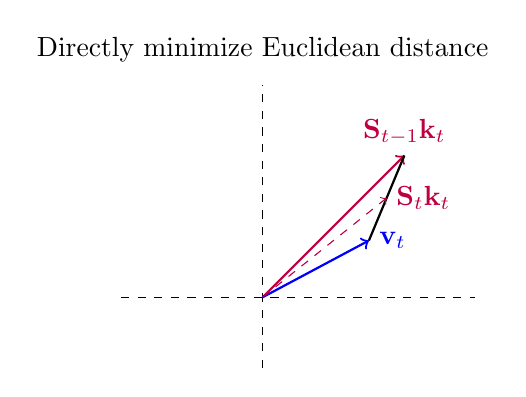
\begin{tikzpicture}[scale=0.9]
            \begin{scope}[xshift=1cm]  
                \node at (0,3.5) {Directly minimize Euclidean distance};
                
                \coordinate (O) at (0,0);
                \draw[dashed] (-2,0) -- (3,0);     
                \draw[dashed] (0,-1) -- (0,3);     
                
                % Original vectors - 调整位置使更分散
                \draw[->,purple,thick] (O) -- (2,2) coordinate (Mk1) node[above] {$\mathbf{S}_{t-1}\mathbf{k}_t$};
                \draw[->,blue,thick] (O) -- (1.5,0.8) coordinate (v) node[right] {$\mathbf{v}_t$};
                
                % Draw the distance line - 需要更新坐标以匹配新的向量位置
                \draw[thick] (2,2) -- (1.5,0.8);
                
                % Dashed vector halfway between Mk1 and v - 调整位置
                \draw[->, purple,dashed] (O) -- (1.75,1.4) node[right] {$\mathbf{S}_{t}\mathbf{k}_t$};
            \end{scope}
        \end{tikzpicture}
     \end{center}
\vspace{-10mm}      
% DeltaNet (\cite{Schlag2021LinearTA, yang2024parallelizing}) optimizes a regression loss via SGD:
    \begin{align*}
        \textbf{Objective: } & \mathcal{L}_t(\mathbf{S}) = \frac{1}{2}\|\mathbf{S} \mathbf{k}_t - \mathbf{v}_t\|^2 \\[1ex]
        \textbf{SGD update: } & \mathbf{S}_t = \mathbf{S}_{t-1} - \beta_t \nabla \mathcal{L}_t(\mathbf{S}_{t-1}) = \mathbf{S}_{t-1} - \beta_t (\mathbf{S}_{t-1} \mathbf{k}_t - \mathbf{v}_t)\mathbf{k}_t^\top 
    \end{align*}
    \vspace{-3mm}

        \begin{itemize}
            \item {\color{red} Better numerical stability}: the norm of $\mathbf{S}_t$ is controlled.
            \item {\color{red} Better in-context associative recall}: directly optimizes key-value association prediction (\cite{Liu2024LonghornSS})
        \end{itemize}




    % Online regression loss is better for predicting $\mathbf{v}_t$ from $\mathbf{k}_t$ and $\mathbf{S}_{t-1}$.
    %     $$\mathcal{L}_t(\mathbf{S}) = \frac{1}{2}\|\mathbf{S} \mathbf{k}_t - \mathbf{v}_t\|^2$$
    %     \vspace{2mm}
    %     Performing a single step of SGD:
    % $$\begin{aligned}
    % \mathbf{S}_t &= \mathbf{S}_{t-1} - \beta_t \nabla \mathcal{L}_t(\mathbf{S}_{t-1}) \\
    % &= \mathbf{S}_{t-1} - \beta_t \left(\mathbf{S}_{t-1} \mathbf{k}_t - \mathbf{v}_t\right) \mathbf{k}_t^\top
    % \end{aligned}$$
    % \begin{itemize}
    %     \item When $\beta_t \in (0, 1)$, the DeltaNet update rule (\cite{Schlag2021LinearTA, yang2024parallelizing}) is recovered.  
    % \end{itemize}
\end{frame}

% \begin{frame}{Comparison between DeltaNet and Linear Attention}
%     \begin{tikzpicture}
%         % Title
%         % Left diagram
%         \begin{scope}[xshift=-4cm]
%             \node at (0,3.5) {Maximize ``alignment''};
%             \node at (0,3) {= Minimize angle + enlarge $|Mk|$};
            
%             % Define coordinates and draw vectors with names
%             \coordinate (O) at (0,0);
%             \draw[->,purple,thick] (O) -- (1.75,1.75) coordinate (Mk) node[above] {$\mathbf{S}_{t-1}\mathbf{k}_t$};
%             \draw[->,green,thick] (O) -- (1.5,0.8) coordinate (v) node[right] {$\mathbf{v}_t$};
            
%             % Add dashed extension to show enlarging norm
%             \draw[->, purple,dashed] (O) -- (3,2.1) node[above] {$\mathbf{S}_{t}\mathbf{k}_t$};
%             % \node[right] at (2.0,2.0) {$\uparrow$};
    
%             % Coordinate axes
%             \draw[dashed] (-1,0) -- (2,0);
%             \draw[dashed] (0,-1) -- (0,2);
            
%             % Draw angle arc
%             \pic [draw, angle radius=5mm] {angle = v--O--Mk};
            
%             % Loss function
%             \node at (0,-1.5) {$\text{loss}_M(k,v) = -\langle \mathbf{S}_{t-1}\mathbf{k}_t, \mathbf{v}_t \rangle$};
%         \end{scope}
        
%         % Right diagram
%         \begin{scope}[xshift=2cm]
%             \node at (0,3.5) {Minimize (Euclidean) distance};
            
%             \coordinate (O) at (0,0);
%             \draw[dashed] (-1,0) -- (2,0);
%             \draw[dashed] (0,-1) -- (0,2);
            
%             % Original vectors
%             \draw[->,purple,thick] (O) -- (1.75,1.75) coordinate (Mk1) node[above] {$\mathbf{S}_{t-1}\mathbf{k}_t$};
%             \draw[->,green,thick] (O) -- (1.5,0.8) coordinate (v) node[right] {$\mathbf{v}_t$};
            
%             % Draw the distance line
%             \draw (1.75,1.75) -- (1.5,0.8);
            
%             % Dashed vector halfway between Mk1 and v
%             \draw[->, purple,dashed] (O) -- (1.6,1.3) node[right] {$\mathbf{S}_{t}\mathbf{k}_t$};
            
%             \node at (0,-1.5) {$\mathcal{L}_{S}(k,v) = \frac{1}{2}\|\mathbf{S}_{t-1}\mathbf{k}_t - \mathbf{v}_t\|^2$};
%         \end{scope}
%     \end{tikzpicture}
%     \begin{itemize}
%         \item Linear attention's objective encourages expanding the norm of $\mathbf{S}_t$, leading to numerical instabilities. 
%         \begin{itemize}
%             \item Weight decay (e.g., in Mamba2) could mitigate this issue.
%         \end{itemize}
%         \item DeltaNet's objective encourages minimizing the distance between $\mathbf{S}_t \mathbf{k}_t$ and $\mathbf{v}_t$, which is more stable.
%     \end{itemize}
% \end{frame}
% \begin{frame}{DeltaNet performs better on in-context associative recall}
%     \begin{block}{Associative recall}
%         \begin{quote}
%             \small ``In psychology, associative memory is {\color{red} \textbf{the ability to learn and remember relationships between unrelated items}}, such as remembering someone's name when seeing their face. This allows us to form connections between distinct pieces of information.''
%         \end{quote}
%     \end{block}
    
%     DeltaNet learns associations through online linear regression: minimizing $\|\mathbf{S}\mathbf{k}_i - \mathbf{v}_i\|^2$ directly optimizes key-value prediction (\cite{Liu2024LonghornSS}).
% \end{frame}

\begin{frame}{In-context associative recall}
    \begin{block}{\scriptsize Multi-Query Associative Recall (MQAR, \cite{zoology})}
        \scriptsize
        A synthetic benchmark for testing in-context associative recall.
        \vspace{1mm}
        \textbf{Example:}
        \begin{itemize}
            \item Given key-value pairs: ``A 4 B 3 C 6 F 1 E 2''
            \item Query: ``A ? C ? F ? E ? B ?''  
            \item Expected output: ``4, 6, 1, 2, 3''
        \end{itemize}
    \end{block}
    \vspace{-1mm}
    
% \definecolor{color1}{RGB}{145,30,180}
% \definecolor{color2}{RGB}{245,130,48}
% \definecolor{color3}{RGB}{230,25,75}
% \definecolor{color4}{RGB}{123,25,75}
% \definecolor{color5}{RGB}{44,160,44}

\definecolor{color1}{RGB}{116, 184, 22}
\definecolor{color2}{RGB}{77, 171, 247}
\definecolor{color3}{RGB}{99, 230, 190}
\definecolor{color4}{RGB}{132, 94, 247}
\definecolor{color5}{RGB}{250, 176, 5}

\begin{figure}
    \centering
    \resizebox{.5\columnwidth}{!}{  
        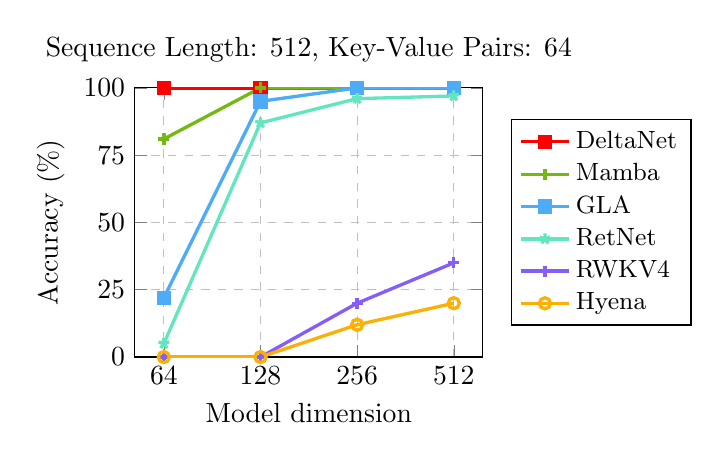
\begin{tikzpicture}
        \begin{axis}[
            name=plot2,
            sharp plot,
            title style={align=right},
            title={Sequence Length: 512, Key-Value Pairs: 64},
            xmode=normal,
            xlabel=Model dimension,
            width=6cm, height=5cm,
            ymin=0, ymax=100,
            symbolic x coords={64,128,256,512},
            ytick={0,25,50,75,100},
            yticklabels={0,25,50,75,100},
            xlabel near ticks,
            ylabel near ticks,
            ylabel=Accuracy (\%),
            ymajorgrids=true,
            xmajorgrids=true,
            grid style=dashed,
            legend style={at={(1.6,0.5)},anchor=east, legend cell align=left, font=\small}, 
        ]

        \addplot[very thick, mark=square*, mark options={scale=1}, color=red] plot coordinates {
            (64,100)
            (128,100)
            (256,100)
            (512,100)
        };
        \addlegendentry{DeltaNet} 

        \addplot[very thick,mark=+,mark options={scale=1}, color=color1] plot coordinates { 
            (64,81)
            (128,100)
            (256,100)
            (512,100)
        };
        \addlegendentry{Mamba} 
        
        \addplot[very thick, mark=square*, mark options={scale=1}, color=color2] plot coordinates {
            (64,22)
            (128,95)
            (256,100)
            (512,100)
        };
        \addlegendentry{GLA} 
        
        \addplot[very thick, mark=star, mark options={scale=1}, color=color3] plot coordinates {
            (64,5)
            (128,87)
            (256,96)
            (512,97)
        };
        \addlegendentry{RetNet}  

        \addplot[very thick, mark=+, mark options={scale=1}, color=color4] plot coordinates {
            (64,0)
            (128,0)
            (256,20)
            (512,35)
        };
        \addlegendentry{RWKV4}  

        \addplot[very thick, mark=o, mark options={scale=1}, color=color5] plot coordinates {
            (64,0)
            (128,0)
            (256,12)
            (512,20)
        };
        \addlegendentry{Hyena} 

        \end{axis}
        \end{tikzpicture}
    }
    \vspace{-3.5mm}
    \caption{Accuracy (\%) on MQAR. DeltaNet achieves the perfect recall.} 
    \label{fig:mqar} 
\end{figure}
\end{frame}
% \begin{frame}{DeltaNet performs better on in-context associative recall: MAD results}
%     MAD (\cite{poli_mechanistic_2024}) serves as a more comprehensive benchmark suite than MQAR for evaluating in-context associative recall and learning.
%     \begin{table}
% \resizebox{\linewidth}{!}{
% \begin{tabular}{l|*{6}{c}|c}
% \toprule
% \textbf{Model} & \textbf{Compress} & \cellcolor{red!15}\textbf{Fuzzy} & \cellcolor{red!15}\textbf{In-Context} & \textbf{Memorize} & \cellcolor{red!15}\textbf{Noisy} & \cellcolor{red!15}\textbf{Selective} & \textbf{Average} \\
% & & \cellcolor{red!15}\textbf{Recall} & \cellcolor{red!15}\textbf{Recall} & & \cellcolor{red!15}\textbf{Recall} & \cellcolor{red!15}\textbf{Copy} & \\
% \midrule
% Transformer & 51.6 & \cellcolor{red!15}29.8 & \cellcolor{red!15}94.1 & 85.2 & \cellcolor{red!15}86.8 & \cellcolor{red!15}99.6 & 74.5 \\
% Hyena & 45.2 & \cellcolor{red!15}7.9 & \cellcolor{red!15}81.7 & 89.5 & \cellcolor{red!15}78.8 & \cellcolor{red!15}93.1 & 66.0 \\
% Multihead Hyena \hspace{4mm} & 44.8 & \cellcolor{red!15}14.4 & \cellcolor{red!15}99.0 & 89.4 & \cellcolor{red!15}98.6 & \cellcolor{red!15}93.0 & 73.2 \\
% Mamba & 52.7 & \cellcolor{red!15}6.7 & \cellcolor{red!15}90.4 & 89.5 & \cellcolor{red!15}90.1 & \cellcolor{red!15}86.3 & 69.3 \\
% GLA & 38.8 & \cellcolor{red!15}6.9 & \cellcolor{red!15}80.8 & 63.3 & \cellcolor{red!15}81.6 & \cellcolor{red!15}88.6 & 60.0 \\
% DeltaNet & 42.2 & \cellcolor{red!15}\textbf{35.7} & \cellcolor{red!15}\textbf{100} & 52.8 & \cellcolor{red!15}\textbf{100} & \cellcolor{red!15}\textbf{100} & 71.8 \\
% \bottomrule
% \end{tabular}
% }
% \caption{MAD benchmark results. DeltaNet achieves the best performance in in-context associative recall and copy tasks, however, it somehow underperforms in memorization and compression tasks.}
% \label{tab:mad_results}
% \end{table}
% \end{frame}


\begin{frame}{Transformers and SSMs in TC$^0$}
    \begin{figure}
        \centering
        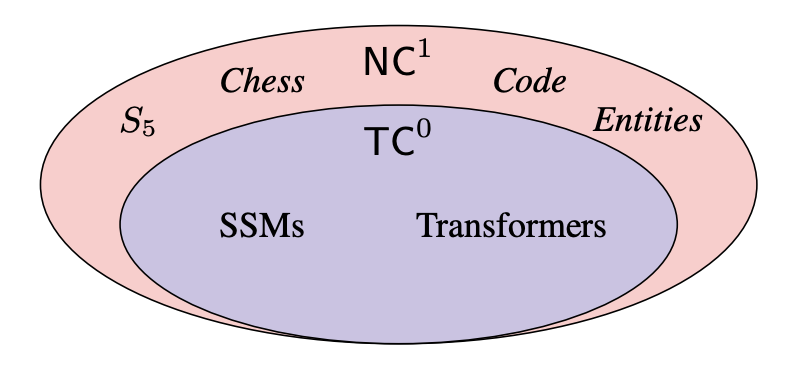
\includegraphics[width=.45\linewidth]{tc0.png}
    \end{figure}
    \vspace{-2mm}
\begin{itemize}
    \item Transformer is in TC$^0$.
    \item Linear RNNs with {\color{red}diagonal transition matrices} (e.g., $\mathbf{S}_t = \mathbf{S}_{t-1} \operatorname{diag}(\boldsymbol{\alpha}_t) + \mathbf{v}_t \mathbf{k}_t^\top$ in GLA) fall under TC$^0$.
    \item {\color{red} Nonlinear RNN} or linear RNN with {\color{red} data-dependent nondiagonal transition matrices} could achieve expressiveness beyond TC$^0$ (\cite{Merrill2024TheIO}).
\end{itemize}
\end{frame}

\begin{frame}{DeltaNet's expressiveness}
    \begin{align*}
    \mathbf{S}_t &= \mathbf{S}_{t-1} - \beta_t \left(\mathbf{S}_{t-1} \mathbf{k}_t - \mathbf{v}_t\right) \mathbf{k}_t^\top \\
    &= \mathbf{S}_{t-1} {\color{blue}\left(\mathbf{I} - \beta_t \mathbf{k}_t \mathbf{k}_t^\top\right)} + \beta_t \mathbf{v}_t \mathbf{k}_t^\top
    \end{align*}

    DeltaNet uses {\color{blue} Generalized Householder} (GH) transition matrices, which are both {\color{red}data-dependent} and {\color{red}nondiagonal}, making it possible to achieve expressiveness beyond $TC^0$.
    % {\color{red}Both conditions} are necessary to achieve expressiveness beyond $TC^0$ (\cite{Merrill2024TheIO}).
\end{frame}



 \begin{frame}{DeltaNet's expressiveness}
    % First show the state update equation
    \begin{align*}
        \mathbf{S}_t &= \mathbf{S}_{t-1} \underbrace{(\mathbf{I} - \beta_t \mathbf{k}_t \mathbf{k}_t^\top)}_{\text{GH transition}} + \beta_t \mathbf{v}_t \mathbf{k}_t^\top 
        = \sum_{i=1}^{t} \left(\beta_i \mathbf{v}_i \mathbf{k}_i^t {\color{blue}\underbrace{\prod_{j=i+1}^{t} (\mathbf{I} - \beta_j \mathbf{k}_j \mathbf{k}_j^\top)}_{\text{cumulative GH products}}}\right)
    \end{align*}

    \vspace{-8mm}
    
    \textbf{Key Properties:}
    \begin{itemize}
        
        \item \textbf{Expressiveness}: When allowing negative eigenvalues in GH matrices (\cite{Grazzi2024UnlockingSI}), {\color{blue}the cumulative products of GH matrices} can represent \textit{any} matrix with Euclidean norm < 1.
        
        \item \textbf{Complexity Class}: 
            {\color{blue}Cumulative products of general matrices} cannot be computed in TC$^0$ (\cite{Mereghetti2000ThresholdCF}).

        \item \textbf{Conclusion}: DeltaNet with negative eigenvalues has expressiveness beyond TC$^0$, strictly exceeding SSMs and Transformer.
    \end{itemize}
\end{frame}

    % \begin{frame}{State tracking performance}
    %     % \begin{quote}
    %     %     ``The ability to track the state of a system is a key component of associative memory, allowing for the retrieval of previously learned information. This is particularly important in tasks like associative recall, where the model must recall previously learned associations between different pieces of information.''
    %     % \end{quote}
    
    % \begin{figure}
    %     \centering
    %     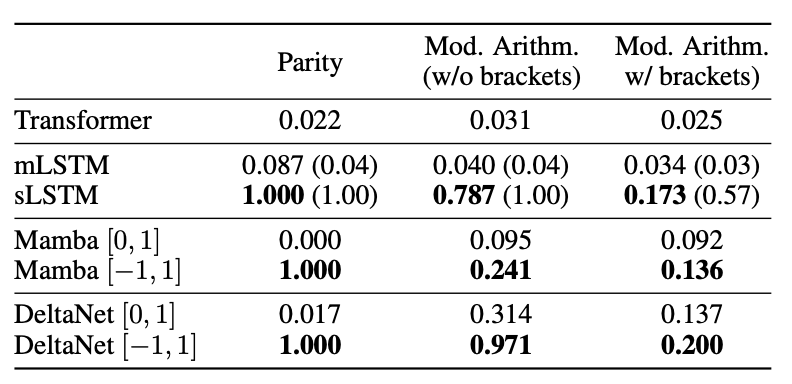
\includegraphics[width=.8\linewidth]{state_tracking.png}
    %     \caption{This table is from \cite{Grazzi2024UnlockingSI}. DeltaNet has a strong state tracking capability in parity checking and modular arithmetic.}
    % \end{figure}
    
    %     \end{frame}
    

\begin{frame}{State tracking performance}
    \begin{figure}
        \centering
        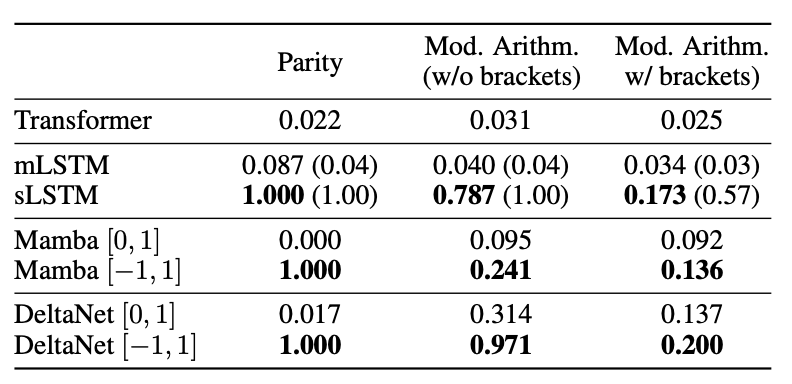
\includegraphics[width=.75\linewidth]{state_tracking.png}
        \caption{State tracking performance comparison (source: \cite{Grazzi2024UnlockingSI}). $[0,1]$ and $[-1,1]$ denotes the ranges of eigenvalues for each model's transition matrix.}
    \end{figure}
    \vspace{-5mm}
   \begin{itemize}
    \item {\color{red}Allowing negative eigenvalues} could boost state tracking performance for both Mamba and DeltaNet.
    \item DeltaNet achieves superior performance due to its {\color{red}richer expressiveness}.
   \end{itemize}
\end{frame}

\begin{frame}{DeltaNet: Chunkwise Parallel Training}
    \begin{align*}
        \mathbf{S}_t &= \mathbf{S}_{t-1} \left(\mathbf{I} - \beta_t \mathbf{k}_t \mathbf{k}_t^\top\right) + \beta_t \mathbf{v}_t \mathbf{k}_t^\top \\
        &= \sum_{i=1}^{t} \left(\beta_i \mathbf{v}_i \mathbf{k}_i^t \underbrace{\prod_{j=i+1}^{t} (\mathbf{I} - \beta_j \mathbf{k}_j \mathbf{k}_j^\top)}_{\mathbf{P}_j^t}\right)
    \end{align*}
    Using the WY representation (\cite{bischof_wy_1985}):
    \[
    \mathbf{P}_{1}^t = \mathbf{I} - \sum_{i=1}^{t}\mathbf{w}_{i}\mathbf{k}_{i}^{\top}.
    \]
    
    {\color{red}\textbf{Key Insight}}: The cumulative product $\prod$ becomes a cumulative sum $\sum$, enabling efficient matrix-multiply-based training.
    \end{frame}

\begin{frame}{DeltaNet: Chunkwise Parallel Training}

    \begin{figure}
        \centering
        \includegraphics[width=.7\linewidth]{delta-chunk.png}
    \end{figure}
    \small
    \vspace{-5mm}
    For more details, please check out our paper or blogpost (https://sustcsonglin.github.io/blog/2024/deltanet-2/).

\end{frame}

% \begin{frame}{DeltaNet can be trained in parallel}
    
%     \begin{figure}
%         \centering
%         \includegraphics[width=0.6\linewidth]{speed.png}
%         \caption{Speed-up of the chunkwise parallel form vs. the recurrent form.}
%     \end{figure}
% When increasing the head dimension and sequence length, chunkwise implementation's speed-up is more significant.
% \end{frame}



 % \begin{frame}{DeltaNet is strictly more expressive than SSMs}
%     % First show the state update equation
%     \begin{align*}
%         \mathbf{S}_t &= \mathbf{S}_{t-1} \underbrace{(\mathbf{I} - \beta_t \mathbf{k}_t \mathbf{k}_t^\top)}_{\text{GH transition}} + \beta_t \mathbf{v}_t \mathbf{k}_t^\top 
%         = \sum_{i=1}^{t} \left(\beta_i \mathbf{v}_i \mathbf{k}_i^t {\color{orange}\underbrace{\prod_{j=i+1}^{t} (\mathbf{I} - \beta_j \mathbf{k}_j \mathbf{k}_j^\top)}_{\text{cumulative GH products}}}\right)
%     \end{align*}

%     \vspace{-3mm}
    
%     \textbf{Key Properties:}
%     \begin{itemize}
        
%         \item \textbf{Expressiveness}: When allowing negative eigenvalues in GH matrices (\cite{Grazzi2024UnlockingSI}), {\color{orange}the cumulative products of GH matrices} can represent \textit{any} matrix with Euclidean norm < 1.
        
%         \item \textbf{Complexity Class}: 
%             {\color{orange}Cumulative products of general matrices} cannot be computed in TC$^0$ (\cite{Mereghetti2000ThresholdCF}).

%         \item \textbf{Conclusion}: DeltaNet with negative eigenvalues has expressiveness beyond TC$^0$, strictly exceeding SSMs and Transformer.
%     \end{itemize}
% \end{frame}

%     \begin{frame}{DeltaNet with negative eigenvalue has better state tracking capability than Transformer and Mamba}
%         % \begin{quote}
%         %     ``The ability to track the state of a system is a key component of associative memory, allowing for the retrieval of previously learned information. This is particularly important in tasks like associative recall, where the model must recall previously learned associations between different pieces of information.''
%         % \end{quote}
    
%     \begin{figure}
%         \centering
%         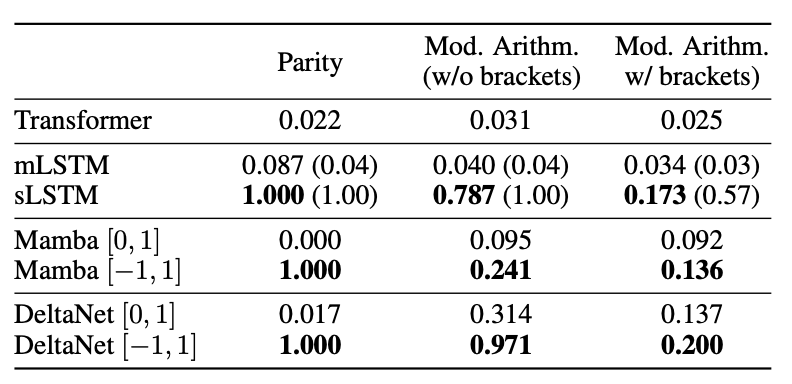
\includegraphics[width=.8\linewidth]{state_tracking.png}
%         \caption{This table is from \cite{Grazzi2024UnlockingSI}. DeltaNet has a strong state tracking capability in parity checking and modular arithmetic.}
%     \end{figure}
    
%         \end{frame}
    

% \begin{frame}{Parallelizing DeltaNet   (\cite{yang2024parallelizing})}
%     By unrolling the recurrence, we can compute the hidden state in parallel for all positions in a chunk.:
%     \begin{align*}
%         \mathbf{S}_t = \sum_{i=1}^{t} \left(\beta_i \mathbf{v}_i \mathbf{k}_i^t \underbrace{\prod_{j=i+1}^{t} (\mathbf{I} - \beta_j \mathbf{k}_j \mathbf{k}_j^\top)}_{\mathbf{P}_j^\top}\right)
%     \end{align*}
% \end{frame}

% \begin{frame}{DeltaNet performs moderately in real-world tasks}
%     DeltaNet: 
%     \begin{itemize}
%         \item[$\smiley$] Strong performance on synthetic benchmarks (e.g., in-context associative recall and state tracking).
%         \item[$\frownie$] Moderate performance in real-world language modeling tasks, overall underperforming Mamba2.
%     \end{itemize}
    

%     \vspace{0.5cm} % Add vertical space for better separation

%     \begin{table}[h!]
%         \centering
%         \resizebox{0.6\linewidth}{!}{%
%             \begin{tabular}{lcccc}
%                 \toprule
%                 \textbf{Model} & \textbf{ppl} $\downarrow$ & \textbf{LM-eval} $\uparrow$ & \textbf{Recall} $\uparrow$ & \textbf{Long} $\uparrow$ \\
%                 \midrule
%                 Mamba1         & 17.92 & 53.12 & 21.0 & \textbf{14.6} \\
%                 Mamba2         & \textbf{16.56} & \textbf{54.89} & \textbf{29.8} & 13.5 \\
%                 DeltaNet       & 17.72 & 52.14 & 26.2 & 13.6 \\
%                 % gated deltanet & 16.42 & 55.32 & 30.6 & 16.6 \\
%                 \bottomrule
%             \end{tabular}
%         }
%         \caption{Performance comparison of different 1.3B models trained on 100B tokens. Source: \cite{yang2024gateddeltanetworksimproving}.}
%         \label{tab:model_comparison}
%     \end{table}
%     \textcolor{red}{Hypothesis: DeltaNet's underperformance may stem from its inability to forget irrelevant information efficiently.} \\
%         \end{frame}


% \begin{frame}{Gated DeltaNet (\cite{yang2024gateddeltanetworksimproving})}
%     Gated DeltaNet combines the delta update rule in DeltaNet and the gated update rule in Mamba2:
%     \begin{align*}
%         \mathbf{S}_t = \mathbf{S}_{t-1} \left({\color{red}\alpha_t}(\mathbf{I} - \beta_t \mathbf{k}_t \mathbf{k}_t^\top)\right) + \beta_t \mathbf{v}_t \mathbf{k}_t^\top
%     \end{align*}
%     \begin{itemize}
%         \item<1-1> ${\color{red}\alpha_t} \in (0, 1)$ is parameterized the same as Mamba2.
%         \item<1-1> When ${\color{red}\alpha_t} = 1$, Gated DeltaNet is equivalent to DeltaNet.
%         \item<1-1> When ${\color{red}\alpha_t} = 0$, Gated DeltaNet clears the entire memory.
%         \item<1-1> Gated DeltaNet can be interpreted as optimizing the online regression loss with weight decay.
%     \end{itemize}
% \end{frame}
% \begin{frame}{Single Needle In a Haystack (S-NIAH)}
%     % \textbf{S-NIAH} is a benchmark suite from \textbf{RULER} (\cite{Hsieh2024RULERWT}) for testing in-context associative recall capabilities through three increasingly challenging subtasks.

%     % \vspace{0.3cm} % 增加垂直间距

%     % \begin{table}[h!]
%     %     \centering
%     %     \scriptsize
%     %     \renewcommand{\arraystretch}{1.2} % 调整行高
%     %     \setlength{\tabcolsep}{4pt} % 调整列间距
%     %     \begin{tabular}{@{}p{1.8cm}|p{3cm}|p{3cm}|p{3cm}@{}}
%     %         \toprule
%     %         \textbf{Task} & \multicolumn{3}{c}{\textbf{Configurations}} \\ 
%     %         \cmidrule(l){2-4}
%     %         & \textbf{Subtask-1} & \textbf{Subtask-2} & \textbf{Subtask-3} \\ 
%     %         \midrule
%     %         Single NIAH &
%     %         \begin{tabular}[t]{@{}l@{}}
%     %             type\_key = word \\ 
%     %             type\_value = number \\ 
%     %             type\_haystack = repeat \\ 
%     %             \textasciitilde passkey retrieval
%     %         \end{tabular} &
%     %         \begin{tabularbiliacat public}[t]{@{}l@{}}
%     %             type\_key = word \\ 
%     %             type\_value = number \\ 
%     %             type\_haystack = essay \\ 
%     %             \textasciitilde vanilla NIAH
%     %         \end{tabular} &
%     %         \begin{tabular}[t]{@{}l@{}}
%     %             type\_key = word \\ 
%     %             type\_value = uuid \\ 
%     %             type\_haystack = essay
%     %         \end{tabular} \\ 
%     %         \bottomrule
%     %     \end{tabular}
%     %     \caption{\scriptsize Configurations for Single NIAH Task}
%     %     \label{tab:single-niah}
%     % \end{table}
% \end{frame}
% % \begin{frame}{Case Study: Single Needle In a Haystack (S-NIAH)}
% %     \begin{block}{S-NIAH-1: Pass-key Retrieval with Synthetic Context}
% %         \scriptsize
% %         \textbf{Context:}
% %         \begin{quote}
% %             A special magic number is hidden within a long text of repeated sentences. Make sure to memorize it. I will quiz you about the number afterwards.

% %             The grass is green. The sky is blue. The sun is yellow. Here we go. There and back again. [....] \textcolor{red}{One of the special magic numbers for flaky-celebrity is: 1538552.} The grass is green. The sky is blue. The sun is yellow. Here we go. There and back again. [....]
% %         \end{quote}

% %         \textbf{Query:} "What is the special magic number for flaky-celebrity?"

% %         \textbf{Expected Answer:} "1538552"
% %     \end{block}
% %     \begin{itemize}
% %         \item<1-> \textbf{Simple Task:} S-NIAH-1 requires memorizing a single number from repetitive context.
% %         \item<1-> \textbf{Repetitive Context:} The model only needs to process the context once, as it is highly redundant.
% %     \end{itemize}
% %     \end{frame}

% % \begin{frame}{Case Study: Single Needle In a Haystack (S-NIAH)}
% %     \centering
% %     \begin{table}
% %         \resizebox{0.6\linewidth}{!}{ % 调整表格宽度
% %             \begin{tabular}{ll|cccc}
% %                 \toprule
% %                 & & \multicolumn{4}{c}{\textbf{S-NIAH-1}} \\
% %                 & & \multicolumn{4}{c}{\textbf{(Pass-key Retrieval)}} \\
% %                 \cmidrule{3-6}
% %                 \textbf{Model} & & \textbf{1K} & \textbf{2K} & \textbf{4K} & \textbf{8K} \\
% %                 \midrule
% %                 DeltaNet       & & 97.4 & 96.8 & \textbf{99.0} & \textbf{98.8} \\
% %                 Mamba2         & & \textbf{99.2} & \textbf{98.8} & 65.4 & 30.4 \\
% %                 Gated DeltaNet & & 98.4 & 88.4 & 91.4 & 91.8 \\
% %                 \bottomrule
% %             \end{tabular}
% %         }
% %         \caption{Performance on S-NIAH-1 task across different sequence lengths. Higher values indicate better performance.}
% %         \label{tab:sniah}
% %     \end{table}
% %     % \vspace{0.1cm} % 增加一点垂直间距
% %     \raggedright
% %     \large \textcolor{red}{\textbf{Key Observation: Decay hurts memory retention!}} \\
% %     \normalsize
% %     \begin{itemize}
% %         \item<1-> Mamba2: Significant drop with longer sequences (decay issue).
% %         \item<1-> DeltaNet: Consistent high performance (robust retention).
% %         \item<1-> Gated DeltaNet: Moderate drop (balanced decay and retention).
% %     \end{itemize}
% %     \end{frame}

% %     \begin{frame}{Case Study: Single Needle In a Haystack (S-NIAH)}
% %         \begin{block}{S-NIAH-2: Number in a Haystack}
% %             \scriptsize
% %             \textbf{Context:}
% %             \begin{quote}
% %                 A special magic number is hidden within the following text. Make sure to memorize it. I will quiz you about the number afterwards.
    
% %                 What hard liquor, cigarettes, heroin, and crack have in common is that they're all more concentrated forms of less addictive predecessors. Most if not all the things we describe as addictive are. [....] \textcolor{red}{One of the special magic numbers for vague-ecology is: 6440561.} And the scary thing is, the process that created them is accelerating. We wouldn't want to stop it. It's the same process that cures diseases: technological progress. Technological progress means making things do more of what we want. When the thing we want is something we want to want, we consider technological progress good [....]
% %             \end{quote}
    
% %                 \textbf{Query:} "What is the special magic number for vague-ecology?"
    
% %                 \textbf{Expected Answer:} "6440561"
% %         \end{block}
    
% %         \begin{itemize}
% %             \item S-NIAH-2 is more {\color{red}{\textbf{challenging}}} than S-NIAH-1, as the context is drawn from Paul Graham Essays rather than synthetic text.
% %             \item Success on this task requires models to \textcolor{red}{\textbf{effectively filter out irrelevant information}}.
% %         \end{itemize}
% %     \end{frame}
    
% %     \begin{frame}{Case Study: Single Needle In a Haystack (S-NIAH)}
% %         \centering
% %         \begin{table}
% %             \resizebox{0.6\linewidth}{!}{ % 调整表格宽度
% %                 \begin{tabular}{ll|cccc}
% %                     \toprule
% %                     & & \multicolumn{4}{c}{\textbf{S-NIAH-2}} \\
% %                     & & \multicolumn{4}{c}{\textbf{(Number in Haystack)}} \\
% %                     \cmidrule{3-6}
% %                     \textbf{Model} & & \textbf{1K} & \textbf{2K} & \textbf{4K} & \textbf{8K} \\
% %                     \midrule
% %                     DeltaNet       & & 98.4 & 45.6 & 18.6 & 14.4 \\
% %                     Mamba2         & & 99.4 & 98.8 & 56.2 & 17.0 \\
% %                     Gated DeltaNet & & \textbf{100.0} & \textbf{99.8} & \textbf{92.2} & \textbf{29.6} \\
% %                     \bottomrule
% %                 \end{tabular}
% %             }
% %             \caption{Performance on S-NIAH-2 task across different sequence lengths. Higher values indicate better performance.}
% %             \label{tab:sniah2}
% %         \end{table}
    
% %         % \vspace{0.3cm} % 增加一点垂直间距
    
% %         \raggedright
% %         \large \textcolor{red}{\textbf{Key Observation: Data-dependent decay helps filter out irrelevant information!}} \\
% %         \normalsize
% %         \begin{itemize}
% %             \item<1-> DeltaNet's performance drops significantly due to lack of decay mechanism.
% %             \item<1-> Mamba2 shows comparable performance to S-NIAH-1 task.
% %             \item<1-> Gated DeltaNet demonstrates superior performance in S-NIAH-2.
% %         \end{itemize}
% %     \end{frame}


% %     \begin{frame}{Case Study: Single Needle In a Haystack (S-NIAH)}
% %         \begin{block}{S-NIAH-3: UUID in a Haystack}
% %             \scriptsize
% %             \textbf{Context:}
% %             \begin{quote}
% %                 A special magic UUID is hidden within the following text. Make sure to memorize it. I will quiz you about the UUID afterwards.
    
% %                 What hard liquor, cigarettes, heroin, and crack have in common is that they're all more concentrated forms of less addictive predecessors. Most if not all the things we describe as addictive are. [....] \textcolor{red}{One of the special magic UUIDs for vague-ecology is: 8a14be62-295b-4715-8333-e8615fb8d16c.} And the scary thing is, the process that created them is accelerating. We wouldn't want to stop it. It's the same process that cures diseases: technological progress. Technological progress means making things do more of what we want. When the thing we want is something we want to want, we consider technological progress good [....]
    
% %             \end{quote}
% %             \textbf{Query:} "What is the special magic UUID for vague-ecology?"
    
% %             \textbf{Expected Answer:} "8a14be62-295b-4715-8333-e8615fb8d16c"

% %         \end{block}
    
% %         \begin{itemize}
% %             \item<1-> S-NIAH-3 is more challenging than S-NIAH-2, as the value is a UUID (a more complex pattern) rather than a number.
% %         \end{itemize}
% %     \end{frame}
% %     \begin{frame}{Case Study: Single Needle In a Haystack (S-NIAH)}
% %         \centering
% %         \begin{table}
% %             \resizebox{0.6\linewidth}{!}{ % 调整表格宽度
% %                 \begin{tabular}{ll|ccc}
% %                     \toprule
% %                     & & \multicolumn{3}{c}{\textbf{S-NIAH-3}} \\
% %                     & & \multicolumn{3}{c}{\textbf{(UUID in Haystack)}} \\
% %                     \cmidrule{3-5}
% %                     \textbf{Model} & & \textbf{1K} & \textbf{2K} & \textbf{4K} \\
% %                     \midrule
% %                     DeltaNet       & & 85.2 & 47.0 & 22.4 \\
% %                     Mamba2         & & 64.4 & 47.6 & 4.6 \\
% %                     Gated DeltaNet & & \textbf{86.6} & \textbf{84.2} & \textbf{27.6} \\
% %                     \bottomrule
% %                 \end{tabular}
% %             }
% %             \caption{Performance on S-NIAH-3 task across different sequence lengths. Higher values indicate better performance.}
% %             \label{tab:sniah3}
% %         \end{table}
    
% %         % \vspace{0.5cm} % 增加垂直间距
    
% %         \raggedright
% %         \large \textcolor{red}{\textbf{Key Observation: Delta rule helps memorize more complex patterns!}} \\
% %         \normalsize
% %         \begin{itemize}
% %             \item<1-> Mamba2's performance drops significantly due to the lack of delta rule.
% %             \item<1-> DeltaNet's performance is similar to S-NIAH-2.
% %             \item<1-> Gated DeltaNet achieves the best performance in S-NIAH-3.
% %         \end{itemize}
% %     \end{frame}

\begin{frame}{Gated DeltaNet}
    Enhancing DeltaNet with {\color{red}{Mamba2-like gating mechanism}} could boost performance on real-world tasks.
        \begin{align*}
            \mathbf{S}_t = \mathbf{S}_{t-1} \left({\color{red}\alpha_t}(\mathbf{I} - \beta_t \mathbf{k}_t \mathbf{k}_t^\top)\right) + \beta_t \mathbf{v}_t \mathbf{k}_t^\top
        \end{align*}
    \begin{table}[h!]
        \centering
        \resizebox{0.9\linewidth}{!}{%
            \begin{tabular}{lcccc}
                \toprule
                \textbf{Model} & \textbf{ppl} $\downarrow$ & \textbf{LM-eval} $\uparrow$ & \textbf{Recall} $\uparrow$ & \textbf{Long} $\uparrow$ \\
                \midrule
                Mamba1         & 17.92 & 53.12 & 21.0 & 14.6 \\
                Mamba2         & 16.56 & 54.89 & 29.8 & 13.5 \\
                DeltaNet       & 17.72 & 52.14 & 26.2 & 13.6 \\
                Gated Deltanet & \textbf{16.42} & \textbf{55.32} & \textbf{30.6} & \textbf{16.6} \\
                \bottomrule
            \end{tabular}
        }
        \caption{Performance comparison of different 1.3B models trained on 100B tokens. Source: \cite{yang2024gateddeltanetworksimproving}.}
        \label{tab:model_comparison}
    \end{table}
\end{frame}
\begin{frame}{DeltaProduct}
    Multiple gradient descent steps per token, resulting in a {\color{red}{high-rank recurrent update}}.
    \begin{align*}
        \mathbf{S}_t^{(i+1)} &= \mathbf{S}_{t-1} \mathbf{A}_t + \mathbf{B}_t \\
        \mathbf{A}_t &= \prod_{i=1}^{n_h} \left(\mathbf{I} - \beta_t^{(i)} \mathbf{k}_t^{(i)} (\mathbf{k}_t^{(i)})^\top\right) \\
        \mathbf{B}_t &= \sum_{i=1}^{n_h} \beta_t^{(i)} \mathbf{v}_t^{(i)} (\mathbf{k}_t^{(i)})^\top \prod_{j=1}^{i-1} \left(\mathbf{I} - \beta_t^{(j)} \mathbf{k}_t^{(j)} (\mathbf{k}_t^{(j)})^\top\right)
    \end{align*}
    \begin{figure}
        \centering
        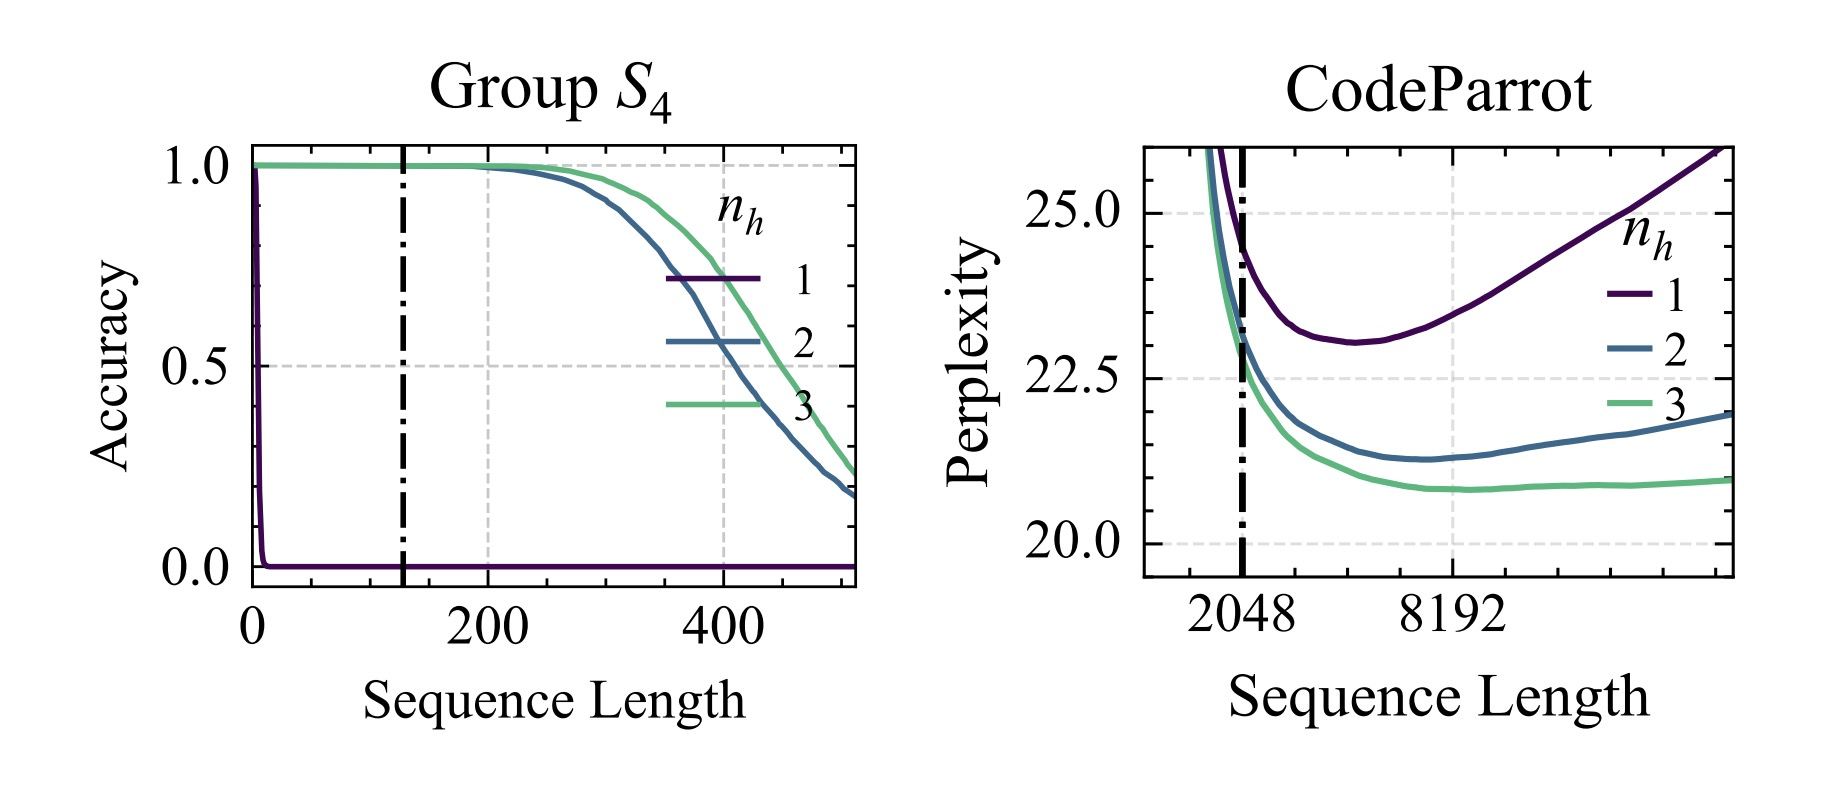
\includegraphics[width=0.65\linewidth]{figure/deltaproduct.jpg}
        \vspace{-4mm}
        \caption{Source: \cite{siems2025deltaproductincreasingexpressivitydeltanet}.}
    \end{figure}
\end{frame}
\begin{frame}{Summary}
    \begin{itemize}
        \item Linear attention and DeltaNet are fast weight programmers with different test-time SGD updates
        \item DeltaNet has strictly more expressive power than Mamba/GLA while maintaining efficient parallelization
        \item Gating and high-rank updates further enhance DeltaNet's performance
    \end{itemize}
\end{frame}


% \begin{frame}{Gated DeltaNet and hybrid models}
% \begin{figure}
%     \centering
%     \includegraphics[width=1\textwidth]{neural-arch.png}
%     \caption{Gated DeltaNet and hybrid blocks. SWA stands for Sliding Window Attention.}
% \end{figure}
% \end{frame}

% \begin{frame}{Zero-shot commonsense reasoning performance}
% \input{figure/common-sense.tex}
% \end{frame}

% \begin{frame}{Zero-shot long context understanding performance}
% \input{figure/longbench.tex}
% \begin{itemize}
%     \item Transformer performs poorly due to limited length extrapolation without long sequence post-training.
% \end{itemize}
% \end{frame}

% \begin{frame}{Zero-shot real-world recall-intensive task performance on short sequences}
%     \input{figure/recall_intensive.tex}
%     \begin{itemize}
%         \item Gated DeltaNet is slightly better than Mamba2 on short sequences. We expect larger performance gap on longer sequences.
%     \end{itemize}
%     \end{frame}

% \begin{frame}{Length extrapolation performance}
%     \begin{figure}
%         \centering
%         \includegraphics[width=0.9\linewidth]{length_extrapolate.png}
%     \end{figure}
% \end{frame}
    

    
% \begin{frame}{Parallelizing (Gated) DeltaNet}
%     \begin{align*}
%         \mathbf{S}_t &= \mathbf{S}_{t-1} \left(\mathbf{I} - \beta_t \mathbf{k}_t \mathbf{k}_t^\top\right) + \beta_t \mathbf{v}_t \mathbf{k}_t^\top \\
%         &= \sum_{i=1}^{t} \left(\beta_i \mathbf{v}_i \mathbf{k}_i^t \underbrace{\prod_{j=i+1}^{t} (\mathbf{I} - \beta_j \mathbf{k}_j \mathbf{k}_j^\top)}_{\mathbf{P}_j^t}\right)
%     \end{align*}
%     $\mathbf{S}_t$ and $\mathbf{P}_t := \mathbf{P}_1^t$ can be computed efficiently via the classical WY representation (\cite{bischof_wy_1985}):
%     \begin{align*}
%         \mathbf{P}_{t} &= \mathbf{I} - \sum_{i=1}^{t}\mathbf{w}_{i}\mathbf{k}_{i}^{\top}, & \mathbf{w}_{t} &= \beta_{t} \left(\mathbf{k}_{t} - \sum_{i=1}^{t-1} \mathbf{w}_{i} (\mathbf{k}_{i}^{\top}\mathbf{k}_{t}) \right) \\
%         \mathbf{S}_t &= \sum_{i=1}^{t}\mathbf{u}_{i} \mathbf{k}_{i}^{\top}, & \mathbf{u}_{t} &= \beta_{t} \left(\mathbf{v}_{t} - \sum_{i=1}^{t-1} \mathbf{u}_{i} (\mathbf{k}_{i}^{\top}\mathbf{k}_{t}) \right)
%     \end{align*}
% \end{frame}

% \begin{frame}{Parallelizing DeltaNet (\cite{yang2024parallelizing})}

%     \begin{figure}
%         \centering
%         \includegraphics[width=.7\linewidth]{delta-chunk.png}
%     \end{figure}
%     \small
%     \vspace{-5mm}
%     Check out our paper or blogpost (https://sustcsonglin.github.io/blog/2024/deltanet-2/) for more details.
%     Gated DeltaNet can be parallelized in a similar manner.
% \end{frame}

% \begin{frame}{Parallelizing DeltaNet (\cite{yang2024parallelizing})}
    
%     \begin{figure}
%         \centering
%         \includegraphics[width=0.6\linewidth]{speed.png}
%         \caption{Speed-up of the chunkwise parallel form vs. the recurrent form.}
%     \end{figure}
% When increasing the head dimension and sequence length, chunkwise implementation's speed-up is more significant.
% \end{frame}

% \begin{frame}{Parallelizing DeltaNet (\cite{yang2024parallelizing})}
%     \begin{figure}
%         \centering
%         \includegraphics[width=0.6\linewidth]{speed-2.png}
%         \caption{Training throughput of 1.3B models on a single H100.}
%     \end{figure}
%     DeltaNet has similar training throughput to GLA, despite its more expressive recurrence.
% \end{frame}
% \begin{frame}{DeltaNet can only modify a single key-value pair at a time}
%     DeltaNet's update rule can be viewed as replacing an old key-value pair with a new one in a soft manner.
%     \begin{align*}
%         \mathbf{v}_t^{\text{old}} &= \mathbf{S}_{t-1} \mathbf{k}_t \\
%         \mathbf{v}_t^{\text{new}} &=  (1-\beta_t) \mathbf{v}_t^{\text{old}} + \beta_t \mathbf{v}_t\\
%         \mathbf{S}_t &=  \mathbf{S}_{t-1} - \beta_t\left(\mathbf{S}_{t-1} \mathbf{k}_t - \mathbf{v}_t\right) \mathbf{k}_t^\top 
%         \\ &= \mathbf{S}_{t-1} - \underbrace{\mathbf{v}_t^{\text{old}} \mathbf{k}_t^\top}_{\text{remove old}} + \underbrace{\mathbf{v}_t^{\text{new}} \mathbf{k}_t^\top}_{\text{write new}}
%     \end{align*}
% \begin{itemize}
%     \item When $\beta_t = 0$, the memory content is intact
%     \item When $\beta_t = 1$, the old key-value pair is completely replaced by the new one.
% \end{itemize}
% % \end{frame}

% \begin{frame}{Chunkwise training for (Gated) DeltaNet}
%     \definecolor{yellowgreen}{RGB}{154, 205, 50}
%     \begin{align*}
%         \mathbf{S}_t &= \mathbf{S}_{t-1}\left(\alpha_t\left(\mathbf{I} - \beta_t \mathbf{k}_t \mathbf{k}_t^\top\right)\right) + \beta_t \mathbf{v}_t \mathbf{k}_t^\top 
%     \\ 
%         &=\sum_{i=1}^t (\beta_i \mathbf{v}_i \mathbf{k}_i^\intercal {\color{black}\underbrace{ \prod_{j=i+1}^t \alpha_j(\mathbf{I} - \beta_j \mathbf{k}_j \mathbf{k}_j^\intercal) }_{\textbf{defined as: } \mathbf{P}_i^t}} ) 
%        % =  \sum_{i=i}^\top \beta_i \mathbf{v}_i \mathbf{k}_i^\intercal \mathbf{P}_i^t
%     \vspace{-20mm}
%     \end{align*}
%      allows for \emph{extended WY representation} where  $\gamma_t:=\prod_{i=1}^t \alpha_i$
%     \begin{align*}
%         &{\color{black}\mathbf{P}_{t} = \color{brown} \gamma_t \color{black}\left( \mathbf{I} - \sum_{i=1}^{t}\mathbf{w}_{i}\mathbf{k}_{i}^{\intercal} \right)}, &&\mathbf{w}_{t} = \beta_{t} \left(\mathbf{k}_{t} -  \sum_{i=1}^{t-1} \mathbf{w}_{i} (\mathbf{k}_{i}^{\intercal}\mathbf{k}_{t})  \right) \\ &{\color{black}\mathbf{S}_t =  \sum_{i=1}^{t} {\color{brown}\frac{\gamma_i}{\gamma_t}}\mathbf{u}_{i} \mathbf{k}_{i}^{\intercal}}, &&
%         \mathbf{u}_{t} = \beta_{t} \left(\mathbf{v}_{t} -  \sum_{i=1}^{t-1} \mathbf{u}_{i} {\color{brown}\frac{\gamma_i}{\gamma_t}}(\mathbf{k}_{i}^{\intercal}\mathbf{k}_{t})  \right)
%     \end{align*}

%     The overheads of gating term is negligible and Gated DeltaNet is as fast as DeltaNet.
% \end{frame}

% \begin{frame}{Chunkwise training for Gated DeltaNet}

%     \begin{figure}
%         \centering
%         \includegraphics[width=0.75\linewidth]{throughputs.png}
%         \caption{Training throughput of 1.3B models on a single H100.}
%     \end{figure}
% \begin{itemize}
%     \item Gated DeltaNet 
%     \item Gated DeltaNet is only slightly slower than Mamba2.
%     \item Hybrid models have higher training throughput thanks to highly optimized flashattention kernel with sliding window size 2K.
% \end{itemize}
% \end{frame}
% \begin{frame}{Chunkwise training for Gated DeltaNet}
%     This chunkwise algorithm can be further extended to the following linear recurrence with diagonal-plus-low-rank transition:
%     \begin{align*}
%         \mathbf{S}_t = \mathbf{S}_{t-1} (\mathbf{D}_t + \boldsymbol{\alpha}_t \boldsymbol{\beta}_t^\top) + \mathbf{v}_t \mathbf{k}_t^\top
%     \end{align*}
%     \begin{itemize}
%         \item $\mathbf{D}_t \in \mathbb{R}^{d \times d}$ is a diagonal matrix. $\boldsymbol{\alpha}_t,\boldsymbol{\beta}_t \in \mathbb{R}^{d}$ are vectors.
%         \item RWKV-7 used such a linear recurrence and has been shown to be effective.
%         \item Fast implementation is available in the flash-linear-attention library (\url{https://github.com/fla-org/flash-linear-attention/blob/main/fla/ops/rwkv7/chunk.py}).
%     \end{itemize}
% \end{frame}



\begin{frame}{}
    \centering
    \LARGE
     Beyond linear regression objective
\end{frame}


\begin{frame}{Beyond linear regression objective}
      DeltaNet optimizes the online linear regression loss:
    \begin{align*}
      \mathcal{L}_t(\mathbf{S}) = \frac{1}{2}\|\mathbf{S} \mathbf{k}_t - \mathbf{v}_t\|^2
    \end{align*}
    \begin{itemize}
        \item This optimization objective assumes linear relationships in historical data dependencies
        \item However, generative AI tasks involve complex, nonlinear dependencies
        \item A linear regression loss may be insufficient to capture these rich patterns.
    \end{itemize}
  \end{frame}
  \begin{frame}{Going beyond online linear regression objective}
    TTT (\cite{sun2024learning}) extends this to a nonlinear regression loss:
    \begin{align*}
      \mathcal{L}_t(\mathbf{S}) = \frac{1}{2}\|f_{\mathbf{S}}(\mathbf{k}_t) - \mathbf{v}_t\|^2
    \end{align*}
    where $f_{\mathbf{S}}$ is a nonlinear transformation parameterized by $\mathbf{S}$.

    Examples:
    \begin{itemize}
        \item TTT-linear: 
            \begin{align*}
                f_{\mathbf{S}}(x) = \operatorname{LN}(\mathbf{S}x) + x,
            \end{align*}
        \item TTT-MLP:
            \begin{align*}
                f_{\mathbf{S}}(x) = \operatorname{LN}(\operatorname{MLP}_{\mathbf{S}}(x)) + x
            \end{align*}
    \end{itemize}

    where $\operatorname{LN}$ denotes layer normalization.

    % \begin{itemize}
    %     \item<1-1> \textbf{TTT-linear}: 
    %         \begin{align*}
    %             f_{\mathbf{S}}(x) = \operatorname{LN}(\mathbf{S}x) + x,
    %         \end{align*}
    %         where \(\operatorname{LN}\) denotes layer normalization.
    %         \begin{itemize}
    %             \item \textcolor{red}{\textbf{TTT-linear is a nonlinear RNN}} due to the presence of layer normalization.
    %         \end{itemize}
    
    %     \item<2-2> \textbf{TTT-MLP}:
    %         \begin{align*}
    %             f_{\mathbf{S}}(x) = \operatorname{LN}(\mathbf{S}_2^\top \sigma(\mathbf{S}_1x)) + x,
    %         \end{align*}
    %         where:
    %         \begin{itemize}
    %             \item \( \mathbf{S} = [\mathbf{S}_1 ; \mathbf{S}_2] \) and \( \mathbf{S}_1, \mathbf{S}_2 \in \mathbb{R}^{d \times 4d} \) are analogous to standard MLP layers with an intermediate hidden dimension expansion factor of 4.
    %             \item \( \sigma \) is a nonlinear activation function, and in TTT-MLP, \( \sigma \) is the GeLU activation.
    %         \end{itemize}
    % \end{itemize}
    
  \end{frame}
  \begin{frame}{Beyond Linear Regression Objective}

    The nonlinear loss induces a nonlinear recurrence, posing challenges for parallelization. \\
    \vspace{0.5em}
    \textcolor{red}{\textbf{Solution}}: Mini-batch Gradient Descent
    \begin{itemize}
        \item Minibatch size aligns with chunk size.
        \item Each token within a chunk is treated as an independent training example for parallel processing.
        \item Sequential dependencies are preserved via a lightweight linear recurrence within chunks.
    \end{itemize}
    \vspace{0.5em}
     This approach essentially combines {\color{red}{intra-chunk linear recurrence}} with {\color{red}{inter-chunk nonlinear recurrence}}.
\end{frame}

  \begin{frame}{Beyond linear regression objective}
    TTT (\cite{sun2024learning}) extends this to a nonlinear regression loss:
    \begin{align*}
      \mathcal{L}_t(\mathbf{S}) = \frac{1}{2}\|f_{\mathbf{S}}(\mathbf{k}_t) - \mathbf{v}_t\|^2
    \end{align*}
    where $f_{\mathbf{S}}$ is a nonlinear transformation parameterized by $\mathbf{S}$.

    \begin{itemize}
        \item Titans (\cite{behrouz2024titanslearningmemorizetest}) further enhances TTT by integrating {\color{red}\textbf{momentum}} and {\color{red}\textbf{weight decay}} into the mini-batch SGD update.
    \end{itemize}
  \end{frame}




  \begin{frame}{Summary}
    \begin{itemize}
        \item \textbf{Modern RNNs through the lens of online learning}:
            \begin{itemize}
                \item (Decaying/Gated) Linear attention: Negative inner-product loss.
                \item (Gated) DeltaNet: Linear regression loss.
                \item TTT \& Titans: Nonlinear regression losses.
            \end{itemize}
        
        \item \textbf{Gradient-based optimization techniques prove valuable}:
            \begin{itemize}
                \item Weight decay enables effective forgetting (e.g., Mamba2, Gated DeltaNet).
                \item Momentum improves performance (e.g., Titans).
            \end{itemize}
        
        \item \textbf{Efficient hardware utilization via}:
            \begin{itemize}
                \item Chunkwise training for linear attention.
                \item Hybrid linear/nonlinear approaches across chunks (e.g., TTT \& Titans).
            \end{itemize}
        
        \item \textbf{Promising future}: Bridging optimization and RNN architectures.
    \end{itemize}
\end{frame}


    
% \end{frame}

% \begin{frame}{Case study: MQAR}

% \begin{frame}{}

    
% \end{frame}

% \begin{frame}{Online regression loss}
%     Hopefully this can be more 
% \end{frame}

% \begin{frame}{DeltaNet}
    

% \end{frame}

% \begin{frame}{Gated DeltaNet}

% \end{frame}

% \begin{frame}{RWKV-7}

% \end{frame}

% \begin{frame}{TTT:}

% \end{frame}

% \begin{frame}{Titans:}

% \end{frame}


